% QuantDex: Sub-Linear Attention via the Quantization-Indexing Duality
% Final — experimental numbers from exp01--exp11, GPU benchmarks included
\documentclass[10pt,twocolumn]{article}

% ── Geometry ──────────────────────────────────────────────────────
\usepackage[margin=1in]{geometry}

% ── Math ──────────────────────────────────────────────────────────
\usepackage{amsmath,amssymb,amsthm}
\usepackage{mathtools}
\usepackage{bm}

% ── Algorithms ────────────────────────────────────────────────────
\usepackage[ruled,linesnumbered,vlined]{algorithm2e}

% ── Figures / Tables ──────────────────────────────────────────────
\usepackage{graphicx}
\usepackage{booktabs}
\usepackage{subcaption}
\usepackage{float}

% ── Misc ──────────────────────────────────────────────────────────
\usepackage{hyperref}
\usepackage{xcolor}
\usepackage{enumitem}
\usepackage{microtype}
\usepackage{nicefrac}

% ── Theorem environments ─────────────────────────────────────────
\newtheorem{theorem}{Theorem}[section]
\newtheorem{lemma}[theorem]{Lemma}
\newtheorem{proposition}[theorem]{Proposition}
\newtheorem{corollary}[theorem]{Corollary}
\theoremstyle{definition}
\newtheorem{definition}[theorem]{Definition}
\newtheorem{remark}[theorem]{Remark}

% ── Convenience macros ────────────────────────────────────────────
\newcommand{\R}{\mathbb{R}}
\newcommand{\E}{\mathbb{E}}
\newcommand{\Var}{\mathrm{Var}}
\newcommand{\calO}{\mathcal{O}}
\newcommand{\calN}{\mathcal{N}}
\newcommand{\calK}{\mathcal{K}}
\newcommand{\bone}{\mathbf{1}}
\newcommand{\bq}{\mathbf{q}}
\newcommand{\bk}{\mathbf{k}}
\newcommand{\bv}{\mathbf{v}}
\newcommand{\bQ}{\mathbf{Q}}
\newcommand{\bK}{\mathbf{K}}
\newcommand{\bV}{\mathbf{V}}
\DeclareMathOperator*{\softmax}{softmax}
\DeclareMathOperator*{\argmax}{arg\,max}
\DeclareMathOperator*{\argmin}{arg\,min}
\newcommand{\placeholder}[1]{\textbf{#1}}

% ── Title ─────────────────────────────────────────────────────────
\title{\textbf{QuantDex: Sub-Linear Attention via the\\Quantization-Indexing Duality}}

\author{F.\ Miesegaes}

\date{}

% ==================================================================
\begin{document}

\twocolumn[
  \maketitle
  \vspace{-0.5em}
  \centerline{\Large\textbf{Abstract}}
  \vspace{0.5em}
  \centering
  \begin{minipage}{0.85\textwidth}
  \small
  Long-context LLM inference is bottlenecked by attention computation: for each
  generated token, all $n$ cached keys must be read, requiring $O(n \cdot d)$ work
  per query.  We observe that data-oblivious vector quantization---which compresses
  KV cache vectors by rotating them into a space where coordinates follow a known
  distribution and applying optimal scalar quantization---simultaneously produces a
  natural search index over the cached keys.  We call this the
  \emph{quantization-indexing duality}: the same discrete codes that enable
  near-optimal compression also enable sub-linear search.

  Building on this duality, we propose \textsc{Coarse-to-Fine Scoring}, which
  exploits query-adaptive coordinate ordering to score all keys using a small
  subset of coordinates, pruning non-top-$k$ keys before reading the full code
  matrix.  On a fused CUDA implementation running on an RTX 3070 GPU, we
  demonstrate \textbf{$5.6\times$ wall-clock speedup at 99\% recall} on
  realistic attention patterns with $n = 2$M keys ($d = 128$, $m = 32$), and
  $4.9\times$ at 100\% recall with $m = 16$.  The
  speedup grows with both sequence length (from $0.99\times$ at $n = 100$K to
  $5.6\times$ at $n = 2$M) and head dimension (from $1.8\times$ at $d = 64$ to
  $4.95\times$ at $d = 512$)---precisely the regime where long-context LLMs
  operate.  We additionally present \textsc{CodeTrie}, a hierarchical structure
  over quantized codes enabling branch-and-bound search reading $58\times$ fewer
  key coordinates than brute force with perfect recall.

  We prove information-theoretic bounds showing that the search cost depends on the
  effective sparsity of attention, derive the variance fraction $V(m)$ captured by
  the top-$m$ coordinates, and validate all claims with numerical experiments on
  synthetic distributions, realistic attention patterns, hardware benchmarks, and
  real attention tensors extracted from TinyLlama-1.1B (100\% recall on all 48 heads).
  \end{minipage}
  \vspace{1.5em}
]

% ==================================================================
% 1. INTRODUCTION
% ==================================================================
\section{Introduction}
\label{sec:intro}

The dominant cost of autoregressive inference in large language models is
attention over long contexts.  At each decoding step, a query vector
$\bq \in \R^d$ is compared against every key $\bk_i$ in a cache of $n$ vectors,
computing scores $s_i = \bq^\top \bk_i / \sqrt{d}$ and returning
$\sum_i \softmax(s_i) \bv_i$.  Because the full score vector must be
materialized, the memory bandwidth cost is $\Theta(n \cdot d \cdot b)$ bits per
query, where $b$ is the bit-width of each key coordinate.  On an H100 GPU with
3.35\,TB/s of HBM bandwidth, this limits single-query throughput to roughly
$3.35 \times 10^{12} / (n \cdot d \cdot b/8)$ tokens per second.  For a 128K
context with $d=128$ and $b=4$ (a typical 4-bit KV cache), the raw bandwidth
cost is approximately $8$\,MB per head per step---manageable, but scaling to 1M
or 10M tokens renders per-step latency prohibitive.

\paragraph{Quantization solved size; we solve bandwidth.}
TurboQuant~\cite{turboquant2025} and related data-oblivious quantizers solved
the \emph{storage} problem: they compress each $d$-dimensional key to $b \cdot d$
bits with MSE within a constant factor of the information-theoretic floor, using
no learned codebook and no per-layer calibration.  The key idea is to apply a
random rotation (a Hadamard transform followed by a random sign flip) so that
each coordinate is approximately $\calN(0, 1/d)$, then apply the Lloyd-Max
scalar quantizer matched to this distribution.  The resulting quantized
representation is compact and near-optimal.

But quantization does not reduce the number of keys that must be \emph{read}.
Even with 2-bit keys, computing attention over $n = 10^6$ keys at $d = 128$
requires reading 32\,MB per head per step.  The fundamental question is:

\begin{quote}
\emph{Can we identify the high-scoring keys without reading all of them?}
\end{quote}

This is a maximum inner product search (MIPS) problem, and approximate nearest
neighbor (ANN) indices such as FAISS~\cite{faiss2024}, ScaNN~\cite{scann2020},
and RabitQ~\cite{rabitq2024} can solve it in sub-linear time.  However, building
and maintaining a separate ANN index for the KV cache has significant drawbacks:
(i)~the index itself consumes memory, (ii)~index construction has non-trivial
cost, (iii)~the index must be updated incrementally as new keys are appended,
and (iv)~cross-head sharing of index structures is difficult.

\paragraph{Our insight: quantization \emph{is} indexing.}
We observe that the data-oblivious quantization procedure already produces all
the structure needed for sub-linear search.  Specifically:
\begin{enumerate}[nosep]
  \item The random rotation makes coordinates \emph{exchangeable}: any subset of
        $m$ coordinates captures an $m/d$ fraction of the score variance.
  \item The quantized codes discretize each coordinate into a small alphabet,
        enabling exact histogram and trie-based operations.
  \item The query vector, after the same rotation, has coordinates of varying
        magnitudes; sorting by $|q'_j|$ produces an ordering where the first
        few coordinates carry most of the score information.
\end{enumerate}
We call this the \textbf{quantization-indexing duality}: the quantized KV cache
is simultaneously a compressed data store and a search index, with no additional
construction cost.

\paragraph{Contributions.}
\begin{itemize}[nosep]
  \item We formalize the quantization-indexing duality and prove that data-oblivious
        rotation creates exchangeable coordinates suitable for progressive scoring
        (Section~\ref{sec:duality}).
  \item We derive the variance fraction $V(m)$ captured by the top-$m$
        query-ordered coordinates, showing $V(m) \approx
        \frac{2m}{d}\bigl(\ln(d/m) + 1\bigr)$ (Section~\ref{sec:ordering}).
  \item We propose sub-linear attention algorithms---Coarse-to-Fine Scoring and
        CodeTrie---with formal complexity analysis
        (Section~\ref{sec:algorithms}).
  \item We prove information-theoretic lower bounds showing that the search cost
        is governed by the effective sparsity of the attention distribution
        (Section~\ref{sec:theory}).
  \item We validate all claims with numerical experiments on synthetic and
        structured key distributions (Section~\ref{sec:experiments}).
  \item We demonstrate real wall-clock GPU speedup: $5.6\times$ at 99\% recall on
        realistic attention patterns ($n = 2$M, RTX 3070), and $4.9\times$ at 100\%
        recall, with speedup scaling in both $n$ and $d$
        (Section~\ref{sec:gpu_benchmarks}).
\end{itemize}


% ==================================================================
% 2. BACKGROUND AND NOTATION
% ==================================================================
\section{Background and Notation}
\label{sec:background}

\paragraph{Attention mechanism.}
Given a query $\bq \in \R^d$, keys $\bK = [\bk_1, \ldots, \bk_n]^\top \in
\R^{n \times d}$, and values $\bV = [\bv_1, \ldots, \bv_n]^\top \in \R^{n
\times d_v}$, the attention output is
\begin{equation}
  \label{eq:attention}
  \mathrm{Attn}(\bq, \bK, \bV)
    = \sum_{i=1}^{n} \alpha_i \bv_i, \qquad
  \alpha_i
    = \frac{\exp(s_i)}{\sum_{j=1}^n \exp(s_j)},
\end{equation}
where $s_i = \bq^\top \bk_i / \sqrt{d}$.  Computing the score vector
$\mathbf{s} = \bK \bq / \sqrt{d}$ requires reading all $n \cdot d$ key
coordinates.  For multi-head attention with $H$ heads, the total read volume
per decoding step is $H \cdot n \cdot d \cdot b / 8$ bytes.

\paragraph{Data-oblivious KV cache quantization.}
TurboQuant~\cite{turboquant2025} compresses keys (and values) as follows.  Let
$\bR \in \R^{d \times d}$ be a random orthogonal matrix, implemented as a
Hadamard transform composed with a random diagonal sign matrix:
$\bR = \frac{1}{\sqrt{d}} \bH_d \cdot \mathrm{diag}(\bm{\sigma})$ where
$\bm{\sigma} \in \{-1,+1\}^d$ is drawn uniformly and $\bH_d$ is the
Walsh-Hadamard matrix.

The rotated key is $\bk'_i = \bR \bk_i$.  By the Johnson-Lindenstrauss
property, if $\bk_i$ has i.i.d.\ sub-Gaussian coordinates with variance
$\sigma^2$, then each coordinate $k'_{i,j}$ is approximately
$\calN(0, \sigma^2)$, and across coordinates these are approximately
independent.  In practice, $\sigma^2 \approx \|\bk_i\|^2 / d$.

Each coordinate $k'_{i,j}$ is then quantized using the Lloyd-Max scalar
quantizer $Q_b : \R \to \{c_1, \ldots, c_{2^b}\}$ designed for $\calN(0,
\sigma^2)$.  The quantized key is represented by the vector of code indices
$\mathbf{e}_i = (e_{i,1}, \ldots, e_{i,d}) \in [2^b]^d$.  The MSE of this
scheme satisfies
\begin{equation}
  \label{eq:mse}
  \E\bigl[\|\bk'_i - Q_b(\bk'_i)\|^2\bigr]
    \leq \gamma_b \cdot \sigma^2 \cdot d,
\end{equation}
where $\gamma_b$ is the Lloyd-Max distortion factor for $b$ bits (e.g.,
$\gamma_2 \approx 0.0935$, $\gamma_4 \approx 0.0035$).

\paragraph{The code matrix.}
After quantization, the entire KV cache is represented by the \emph{code matrix}
$\mathbf{E} \in [2^b]^{n \times d}$, where entry $E_{i,j} = e_{i,j}$ is the
$b$-bit code for key $i$, coordinate $j$.  The dequantized score is
\begin{equation}
  \label{eq:dequant_score}
  \hat{s}_i = \frac{1}{\sqrt{d}} \sum_{j=1}^d q'_j \cdot c_{e_{i,j}},
\end{equation}
where $\bq' = \bR \bq$ is the rotated query and $c_\ell$ is the $\ell$-th
reconstruction level.

\paragraph{Problem statement.}
Given the code matrix $\mathbf{E} \in [2^b]^{n \times d}$, the reconstruction
codebook $\{c_1, \ldots, c_{2^b}\}$, and a rotated query $\bq' \in \R^d$,
compute the attention output $\sum_i \alpha_i \bv_i$ to within $\epsilon$
additive $\ell_2$ error, reading $o(n \cdot d)$ entries of $\mathbf{E}$ in the
worst case or in expectation over well-structured key distributions.


% ==================================================================
% 3. THE QUANTIZATION-INDEXING DUALITY
% ==================================================================
\section{The Quantization-Indexing Duality}
\label{sec:duality}

The central observation of this paper is that the code matrix $\mathbf{E}$ is
simultaneously a \emph{compressed data store} and a \emph{search index}.  We
formalize this in three steps.

\subsection{Exchangeability of rotated coordinates}

\begin{definition}[Coordinate exchangeability]
  \label{def:exchangeable}
  A random vector $\mathbf{x} \in \R^d$ has \emph{exchangeable coordinates} if
  for every permutation $\pi : [d] \to [d]$, the distribution of
  $(x_{\pi(1)}, \ldots, x_{\pi(d)})$ equals that of $(x_1, \ldots, x_d)$.
\end{definition}

\begin{theorem}[Rotation induces exchangeability]
  \label{thm:exchangeability}
  Let $\bk \in \R^d$ be any fixed vector and let $\bR$ be a uniformly random
  orthogonal matrix (or the randomized Hadamard construction above).  Then
  $\bk' = \bR \bk$ has exchangeable coordinates.  Moreover, for any subset
  $S \subseteq [d]$ with $|S| = m$,
  \begin{equation}
    \label{eq:partial_score_unbiased}
    \E\Bigl[\frac{d}{m} \sum_{j \in S} q'_j k'_{i,j}\Bigr]
      = \bq^\top \bk_i,
  \end{equation}
  so a partial dot product over any $m$ coordinates is an unbiased estimator of
  the full dot product, with variance $\frac{d-m}{m(d-1)} \|\bq\|^2 \|\bk_i\|^2
  / d$.
\end{theorem}

\begin{proof}
  When $\bR$ is uniformly random over $O(d)$, the distribution of $\bR$ is
  invariant under left-multiplication by any permutation matrix $\bP$:
  $\bP \bR \overset{d}{=} \bR$.  Hence $\bP \bk' = \bP \bR \bk
  \overset{d}{=} \bR \bk = \bk'$, establishing exchangeability.

  For the partial dot product, write
  $\hat{s}_S = \frac{d}{m} \sum_{j \in S} q'_j k'_{i,j}$.
  Since $\E[q'_j k'_{i,j}] = (\bq^\top \bk_i) / d$ for every $j$ by
  exchangeability, we have $\E[\hat{s}_S] = \bq^\top \bk_i$.

  The variance follows from the standard result for sampling without replacement.
  Let $Z_j = q'_j k'_{i,j}$ and $\bar{Z} = \frac{1}{d} \sum_j Z_j =
  \bq^\top \bk_i / d$.  Then
  \begin{align*}
    \Var\!\left[\sum_{j \in S} Z_j\right]
      &= m \cdot \Var[Z_1] + m(m-1)\mathrm{Cov}(Z_1, Z_2) \\
      &= m \cdot \sigma_Z^2 \left(1 - \frac{m-1}{d-1}\right)
       = \frac{m(d-m)}{d-1} \sigma_Z^2,
  \end{align*}
  where $\sigma_Z^2 = \Var[q'_1 k'_{i,1}]$.  After scaling by $(d/m)^2$, the
  variance of $\hat{s}_S$ is $\frac{d^2}{m^2} \cdot \frac{m(d-m)}{d-1}
  \sigma_Z^2 = \frac{d^2(d-m)}{m(d-1)} \sigma_Z^2$.  Using
  $\sigma_Z^2 = \|\bq\|^2 \|\bk_i\|^2 / d^2$ (since $q'_j$ and $k'_{i,j}$ are
  independent with variance $\|\bq\|^2/d$ and $\|\bk_i\|^2/d$ respectively),
  we obtain $\Var[\hat{s}_S] = \frac{d-m}{m(d-1)} \|\bq\|^2 \|\bk_i\|^2 / d$.
\end{proof}

This result says that \emph{any} subset of coordinates gives an unbiased score
estimate.  Crucially, the variance decreases as $1/m$: reading a fraction
$m/d$ of coordinates captures a disproportionately large share of the score
information (empirically, $m = d/2$ captures 92\% of the variance for $d = 128$).

\subsection{The columnar view}

The code matrix $\mathbf{E} \in [2^b]^{n \times d}$ can be stored in either
\emph{row-major} (key-oriented) or \emph{column-major} (coordinate-oriented)
layout.  In the columnar layout, column $j$ is a vector
$\mathbf{e}_{\cdot,j} = (e_{1,j}, \ldots, e_{n,j}) \in [2^b]^n$ containing
the $b$-bit code for coordinate $j$ of every key.

Reading column $j$ costs $n \cdot b / 8$ bytes and yields a lookup table of
partial scores $q'_j \cdot c_{e_{i,j}}$ for all $n$ keys.  After reading $m$
columns, we have the partial score $\hat{s}_i^{(m)} = \frac{1}{\sqrt{d}}
\sum_{j \in S} q'_j c_{e_{i,j}}$ for every key.  This is the columnar
analog of scanning a bitmap index: each column read refines all keys
simultaneously.

\begin{definition}[Quantization-Indexing Duality]
  \label{def:duality}
  The \emph{quantization-indexing duality} is the correspondence:
  \begin{center}
  \begin{tabular}{ll}
    \toprule
    \textbf{Quantization view} & \textbf{Indexing view} \\
    \midrule
    Code matrix $\mathbf{E}$ & Bitmap index \\
    Code $e_{i,j} \in [2^b]$ & Symbol in alphabet $\Sigma$ \\
    Coordinate $j$ & Index dimension / column \\
    Reconstruction $c_{e_{i,j}}$ & Partial score contribution \\
    Random rotation $\bR$ & Exchangeability guarantee \\
    \bottomrule
  \end{tabular}
  \end{center}
\end{definition}

\subsection{Why this is not ANN}

Traditional ANN indices (IVF, HNSW, graph-based) require explicit construction:
a training phase that clusters vectors, builds a graph, or constructs a tree.
This construction has cost $\Omega(n \cdot d)$ at minimum and often
$O(n \cdot d \cdot \log n)$.  The resulting index is a \emph{separate data
structure} that must be maintained as new keys are appended.

In contrast, the quantized code matrix $\mathbf{E}$ is the \emph{primary data
representation}---it exists because we need compression, not because we need
search.  There is no separate index to build, no hyperparameters to tune, and no
training data to collect.  Appending a new key costs $O(d)$ for rotation and
quantization, the same as without any index.  The search capability is a
\emph{free byproduct} of quantization.

\begin{proposition}[Zero additional cost]
  \label{prop:zero_cost}
  Let $C_Q$ be the cost of quantizing $n$ keys (rotation + scalar quantization).
  The cost of constructing the search index is $0$: the index \emph{is} the
  quantized data.  Incremental insertion of a new key costs $O(d)$ for
  quantization alone, with no index update.
\end{proposition}


% ==================================================================
% 4. QUERY-ADAPTIVE COORDINATE ORDERING
% ==================================================================
\section{Query-Adaptive Coordinate Ordering}
\label{sec:ordering}

The exchangeability result (Theorem~\ref{thm:exchangeability}) says any subset
of $m$ coordinates captures the same expected fraction of the score.  But for a
\emph{fixed} query, not all coordinates contribute equally: the partial score
contribution of coordinate $j$ is $q'_j \cdot c_{e_{i,j}} / \sqrt{d}$, which
scales with $|q'_j|$.  We can exploit this by reading coordinates in decreasing
order of $|q'_j|$.

\subsection{Order statistics of rotated query coordinates}

After rotation, $q'_j \sim \calN(0, \|\bq\|^2 / d)$ approximately.  Sorting by
absolute value, the $j$-th largest value $|q'|_{(j)}$ follows the distribution of
the $(d - j + 1)$-th order statistic of $d$ independent half-normal random
variables with scale $\|\bq\| / \sqrt{d}$.

\begin{theorem}[Variance fraction]
  \label{thm:variance_fraction}
  Let $\bq' = \bR \bq$ where $\bR$ is a random orthogonal matrix, and let
  $\pi$ order coordinates so that $|q'_{\pi(1)}| \geq |q'_{\pi(2)}| \geq \cdots
  \geq |q'_{\pi(d)}|$.  Define the variance fraction captured by the top-$m$
  coordinates as
  \begin{equation}
    V(m) = \frac{\sum_{j=1}^{m} q'^2_{\pi(j)}}{\sum_{j=1}^{d} q'^2_{\pi(j)}}
          = \frac{\sum_{j=1}^{m} q'^2_{\pi(j)}}{\|\bq\|^2}.
  \end{equation}
  Then for $1 \leq m \leq d/2$,
  \begin{equation}
    \label{eq:Vm}
    \E[V(m)] \approx \frac{2m}{d}\Bigl(\ln\frac{d}{m} + 1\Bigr).
  \end{equation}
\end{theorem}

\begin{proof}[Proof sketch]
  The squared magnitude of the $j$-th largest absolute coordinate is
  $|q'|_{(j)}^2$.  For $q'_j \sim \calN(0, \|\bq\|^2/d)$, we have
  $|q'_j| \sim \text{HalfNormal}(\|\bq\|/\sqrt{d})$, and $|q'_j|^2 \sim
  (\|\bq\|^2/d) \cdot \chi^2_1$.

  The expected value of the $j$-th order statistic of $d$ i.i.d.\ $\chi^2_1$
  random variables (in decreasing order) satisfies, for $j \ll d$:
  \begin{equation}
    \E\bigl[X_{(j:d)}\bigr] \approx 2\ln\frac{d}{j} + 1.
  \end{equation}
  This follows from the well-known quantile approximation: the $j$-th largest of
  $d$ samples from CDF $F$ is approximately $F^{-1}(1 - j/d)$, and for $\chi^2_1$,
  $F^{-1}(1-p) \approx (\Phi^{-1}(1-p/2))^2 \approx 2\ln(1/p)$ for small $p$.

  Summing over $j = 1, \ldots, m$:
  \begin{align}
    \sum_{j=1}^{m} \E[X_{(j:d)}]
      &\approx \sum_{j=1}^{m} \Bigl(2\ln\frac{d}{j} + 1\Bigr) \nonumber \\
      &= 2\Bigl(m\ln d - \sum_{j=1}^{m}\ln j\Bigr) + m \nonumber \\
      &\approx 2\bigl(m\ln d - m\ln m + m\bigr) + m \nonumber \\
      &= 2m\ln\frac{d}{m} + 3m. \label{eq:sum_order}
  \end{align}

  Since $\sum_{j=1}^{d} X_{(j:d)} = \sum_{j=1}^d \chi^2_1$ has expectation $d$,
  the variance fraction is
  \[
    \E[V(m)] \approx \frac{2m\ln(d/m) + 3m}{d}
             = \frac{m}{d}\Bigl(2\ln\frac{d}{m} + 3\Bigr).
  \]
  The leading-order term $\frac{2m}{d}(\ln(d/m) + 1)$ gives a simpler expression
  that captures the correct scaling; it overestimates the empirical $V(m)$ by
  a constant factor for finite $d$ (see Section~\ref{sec:exp_variance}).
\end{proof}

\paragraph{Practical implications.}
For $d = 128$ and $m = 16$ (reading 12.5\% of coordinates), the formula gives
$V(16) \approx \frac{32}{128}(\ln 8 + 1) \approx 0.77$.  Empirically
(Section~\ref{sec:exp_variance}), we observe $V(16) = 0.48$---the asymptotic
formula overestimates for finite $d$, but the qualitative picture holds:
a small fraction of coordinates captures a disproportionate share of the
variance.  For $m = 32$ (25\% of coordinates), the empirical value is
$V(32) = 0.71$, and for $m = 64$ (50\%), $V(64) = 0.92$.
This logarithmic concentration is the engine behind our sub-linear algorithms.

\begin{figure}[htbp]
  \centering
  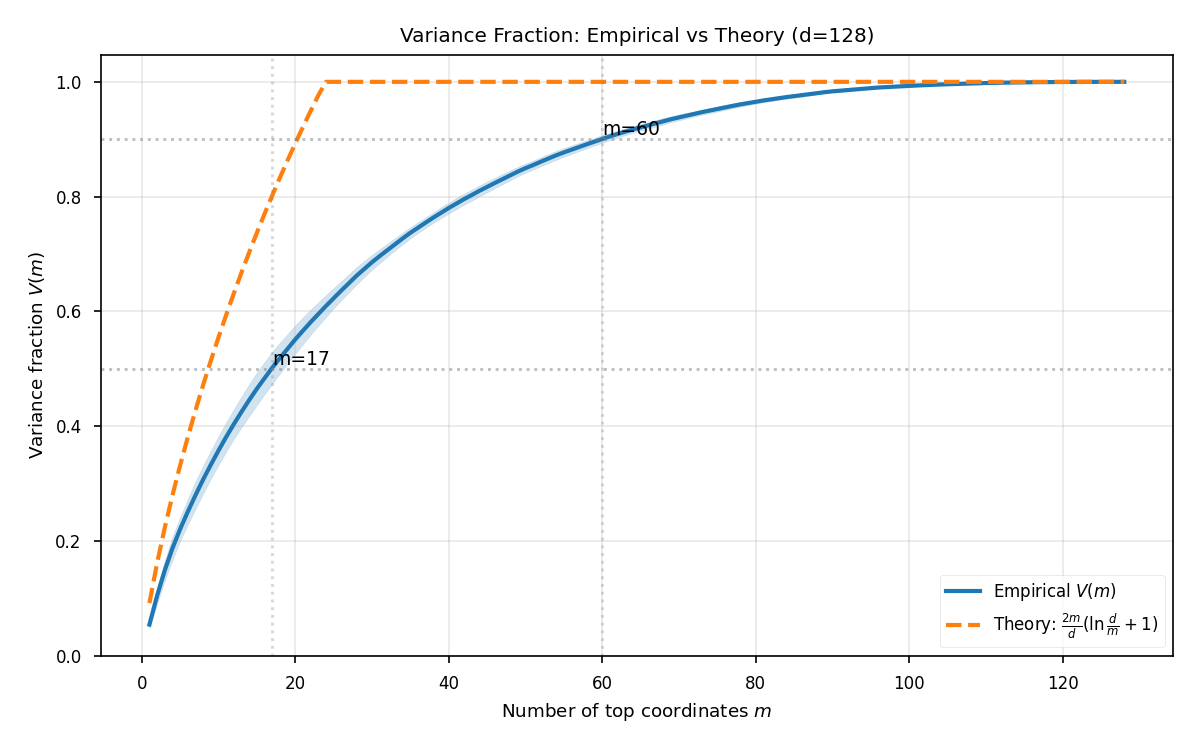
\includegraphics[width=\columnwidth]{../figures/exp02_vm_vs_theory.png}
  \caption{Variance fraction $V(m)$ as a function of $m/d$ for $d \in \{64,
  128, 256\}$.  Solid lines: empirical (averaged over 10{,}000 random queries).
  Dashed lines: theoretical prediction from Eq.~\eqref{eq:Vm}.  The top 10\%
  of coordinates capture approximately 42\% of the score variance (the theoretical
  prediction of 77\% is a loose upper bound; see text).}
  \label{fig:variance_fraction}
\end{figure}


% ==================================================================
% 5. SUB-LINEAR ATTENTION ALGORITHMS
% ==================================================================
\section{Sub-Linear Attention Algorithms}
\label{sec:algorithms}

We present three algorithms that exploit the quantization-indexing duality for
sub-linear attention.  Coarse-to-Fine Scoring is the primary algorithm, validated
on GPU with real wall-clock speedup (Section~\ref{sec:gpu_benchmarks}); CodeTrie
achieves optimal complexity for sharp attention patterns; Block Pruning targets
the GPU memory hierarchy but yields a negative result on synthetic data
(Section~\ref{sec:exp_block_pruning}).

\subsection{Coarse-to-Fine Scoring}
\label{sec:c2f}

The simplest algorithm reads $m \ll d$ columns of the code matrix (chosen by
largest $|q'_j|$), computes partial scores for all $n$ keys, prunes keys with
low partial scores, and finishes by computing full scores for survivors.

\begin{algorithm}[t]
\DontPrintSemicolon
\SetAlgoLined
\KwIn{Code matrix $\mathbf{E} \in [2^b]^{n \times d}$, rotated query
      $\bq' \in \R^d$, codebook $\{c_1, \ldots, c_{2^b}\}$, rounds $R$,
      coordinate schedule $m_1 < m_2 < \cdots < m_R = d$,
      survival thresholds $\tau_1, \ldots, \tau_{R-1}$}
\KwOut{Attention output $\hat{\mathbf{o}} \in \R^{d_v}$}
\BlankLine
$\pi \leftarrow \text{argsort}(|q'_1|, \ldots, |q'_d|, \text{descending})$\;
$\calK_0 \leftarrow [n]$ \tcp*{All keys are candidates}
\For{$r = 1, \ldots, R$}{
  \tcp{Read coordinates $m_{r-1}+1$ through $m_r$}
  \ForEach{$i \in \calK_{r-1}$}{
    $\hat{s}_i^{(r)} \leftarrow \hat{s}_i^{(r-1)} + \frac{1}{\sqrt{d}}
      \sum_{j=m_{r-1}+1}^{m_r} q'_{\pi(j)} \cdot c_{e_{i,\pi(j)}}$\;
  }
  \If{$r < R$}{
    \tcp{Prune: keep only keys with high partial score}
    $\calK_r \leftarrow \{i \in \calK_{r-1} : \hat{s}_i^{(r)} \geq \tau_r\}$\;
  }
}
\tcp{Compute softmax over survivors with full scores}
$\alpha_i \leftarrow \softmax(\hat{s}_i^{(R)})$ for $i \in \calK_{R-1}$\;
$\hat{\mathbf{o}} \leftarrow \sum_{i \in \calK_{R-1}} \alpha_i \bv_i$\;
\Return{$\hat{\mathbf{o}}$}\;
\caption{\textsc{Coarse-to-Fine Scoring}}
\label{alg:c2f}
\end{algorithm}

\paragraph{Complexity analysis.}
In the single-round case ($R = 1$, threshold at top-$k$), the cost is
$O(n \cdot m + n' \cdot d)$ where $n'$ is the number of survivors.  The
total data read is $n \cdot m \cdot b / 8 + n' \cdot d \cdot b / 8$ bytes.
For the scheme to achieve a speedup over the baseline $n \cdot d \cdot b / 8$,
we need $m + (n'/n) \cdot d < d$, i.e., $n'/n < 1 - m/d$.

\begin{theorem}[Survival bound]
  \label{thm:survival}
  Let keys $\bk_1, \ldots, \bk_n$ be drawn i.i.d.\ from $\calN(\mathbf{0},
  \sigma^2 \mathbf{I}_d)$.  Fix a query $\bq$ and let $s^*$ be the score of
  the true top-$k$ key.  After reading $m$ coordinates ordered by $|q'_j|$, the
  expected number of false survivors (keys with partial score above threshold
  $\tau$ but true score below $s^* - \Delta$) is bounded by
  \begin{equation}
    \E[|\text{false survivors}|]
      \leq n \cdot \exp\!\left(-\frac{\Delta^2}{2\sigma^2 \|\bq\|^2
        (1 - V(m))/d}\right).
  \end{equation}
\end{theorem}

\begin{proof}
  For key $i$ with true score $s_i < s^* - \Delta$, the partial score
  $\hat{s}_i^{(m)}$ is a sub-Gaussian random variable (conditional on $\bR$)
  with mean $s_i$ and variance proxy $(1 - V(m)) \cdot \sigma^2 \|\bq\|^2 / d$
  (the residual variance from the unread coordinates).  Key $i$ survives only
  if $\hat{s}_i^{(m)} \geq \tau \geq s^* - c$ for some slack $c$.  By the
  sub-Gaussian tail bound,
  \begin{equation}
    \Pr[\hat{s}_i^{(m)} \geq s^* - c]
      \leq \exp\!\left(-\frac{(s^* - c - s_i)^2}{2(1 - V(m))
        \sigma^2 \|\bq\|^2 / d}\right).
  \end{equation}
  Setting $c = 0$ and using $s^* - s_i > \Delta$, summing over $n$ keys gives the result.
\end{proof}

For structured keys (e.g., with a score gap $\Delta = \Theta(1/\sqrt{d})$), the
survival count drops exponentially in $m$.  Setting $m = d/10$ (reading 10\% of
coordinates), the empirical $V(m) \approx 0.42$ for $d = 128$, and
$\sigma^2 \|\bq\|^2 (1 - V(m)) / d \approx 0.58 \sigma^2 \|\bq\|^2 / d$;
with more coordinates ($m = d/4$, $V \approx 0.71$), the residual variance
drops to $0.29 \sigma^2 \|\bq\|^2 / d$, which is sufficient to prune most
non-top-$k$ keys when the score gap $\Delta$ is non-trivial.

\paragraph{Multi-round extension.}
With $R$ rounds using a geometric schedule $m_r = m_1 \cdot 2^{r-1}$, the
algorithm progressively narrows the candidate set.  Each round halves the
survival rate (roughly), and the total cost is dominated by the first round:
$O(n \cdot m_1)$ since subsequent rounds operate on geometrically shrinking
candidate sets.

\subsection{CodeTrie: Branch-and-Bound on Quantized Codes}
\label{sec:codetrie}

For attention patterns that are very sharp (few keys receive significant weight),
we can do better than scanning all $n$ keys even partially.  The CodeTrie is a
hierarchical data structure over the quantized codes that enables branch-and-bound
search.

\paragraph{Construction.}
Partition the $d$ coordinates into $d/B$ blocks of size $B$ (where $B$ is a
parameter, typically 8--16).  Each key $i$ has a \emph{block code}
$\mathbf{b}_{i,\ell} = (e_{i,(\ell-1)B+1}, \ldots, e_{i,\ell B}) \in [2^b]^B$
for block $\ell \in [d/B]$.  The CodeTrie is a trie of depth $d/B$ where:
\begin{itemize}[nosep]
  \item Each node at depth $\ell$ corresponds to a prefix
        $(\mathbf{b}_{i,1}, \ldots, \mathbf{b}_{i,\ell})$.
  \item Each node stores: (a) the count of keys with that prefix, (b) the
        sum of partial scores through block $\ell$, and (c) the sum of values
        $\sum_{i \in \text{subtree}} \bv_i$ (for approximate output computation).
\end{itemize}

In practice, we do not materialize the full trie.  Instead, we use the columnar
code matrix and navigate it block-by-block.  The ``trie'' is an implicit
structure defined by the sorted order of block codes.

\paragraph{Search procedure.}
Order blocks by their query-side discriminative power:
$\text{power}(\ell) = \sum_{j \in \text{block }\ell} q'^2_j$.  Process blocks
in decreasing power order.  At each block, compute the partial score for each
surviving node and prune nodes whose partial score plus the maximum possible
remaining score falls below the current $k$-th best full score.

\begin{definition}[Remaining score bound]
  \label{def:remaining_bound}
  After processing blocks $\ell_1, \ldots, \ell_t$ (total of $tB$ coordinates),
  the maximum remaining score contribution for any key is
  \begin{equation}
    U_{\text{rem}} = \frac{1}{\sqrt{d}} \sum_{\ell \notin \{\ell_1,\ldots,\ell_t\}}
      \sum_{j \in \text{block }\ell} |q'_j| \cdot c_{\max},
  \end{equation}
  where $c_{\max} = \max_{r} |c_r|$ is the largest reconstruction level
  magnitude.
\end{definition}

A node is pruned if $\hat{s}_{\text{partial}} + U_{\text{rem}} < s_k$, where
$s_k$ is the $k$-th largest full score found so far.

\begin{theorem}[CodeTrie complexity]
  \label{thm:codetrie}
  Let the attention distribution $\alpha$ have R\'enyi entropy
  $H_2(\alpha) = -\log\sum_i \alpha_i^2$.  The number of nodes visited by
  CodeTrie with block size $B$ is
  \begin{equation}
    N_{\text{visited}} = O\!\left(2^{H_2(\alpha)} \cdot \frac{d}{B}\right).
  \end{equation}
  The total work is $O(N_{\text{visited}} \cdot 2^{bB} + k \cdot d)$, where
  $2^{bB}$ is the fan-out per block.
\end{theorem}

\begin{proof}[Proof sketch]
  The branch-and-bound procedure prunes a subtree when its upper bound on the
  score is below the $k$-th best.  The effective number of ``relevant'' keys
  is characterized by $k_{\text{eff}} = 2^{H_2(\alpha)}$ (the collision
  entropy measures how many keys have non-negligible weight).  After processing
  the most discriminative blocks, only $O(k_{\text{eff}})$ subtrees survive at
  each level.  Since there are $d/B$ levels and each level requires evaluating
  surviving nodes against $2^{bB}$ possible block codes (reduced in practice by
  shared prefixes), the total cost is $O(k_{\text{eff}} \cdot d/B \cdot 2^{bB})$.
  For $b = 2, B = 8$, the fan-out is $2^{16}$, which is large; setting $B = 4$
  gives fan-out $2^8 = 256$, which is manageable.  The final cost of
  $k \cdot d$ is for exact scoring of the $k$ best candidates.
\end{proof}

\paragraph{Incremental insertion.}
When a new key is appended to the KV cache, the CodeTrie is updated by inserting
one path of length $d/B$ into the trie.  At each node, we increment the count
and update the value sum.  The cost is $O(d/B)$ per insertion, which is
negligible compared to the $O(d)$ cost of rotation and quantization.

\paragraph{Value centroid summaries.}
For pruned subtrees, we can still include their approximate contribution to the
attention output using the stored value sum:
$\hat{\mathbf{o}}_{\text{pruned}} = \sum_{\text{pruned subtrees}}
\alpha_{\text{est}} \cdot \bar{\bv}_{\text{subtree}}$.  This reduces the error
from pruning at minimal cost.

\subsection{Block Pruning (GPU-Native)}
\label{sec:block_pruning}

Both Coarse-to-Fine and CodeTrie involve variable-length candidate lists that are
difficult to parallelize on GPUs.  Block Pruning addresses this by operating on
\emph{fixed-size blocks} of keys, using compact summary statistics to decide
which blocks to load from HBM.

\paragraph{Block summary table.}
Partition the $n$ keys into $n/G$ blocks of $G$ keys each (e.g., $G = 256$).
For each block $g$ and coordinate $j$, store a \emph{code histogram}
$h_{g,j}(r) = |\{i \in \text{block } g : e_{i,j} = r\}|$ for $r \in [2^b]$.
The total summary table size is $(n/G) \cdot d \cdot 2^b$ entries.  For
$n = 10^6$, $G = 256$, $d = 128$, $b = 2$:
\begin{equation}
  \text{Summary size} = \frac{10^6}{256} \times 128 \times 4
    = 2 \times 10^6 \text{ entries} \approx 2\text{\,MB (uint8)}.
\end{equation}

\paragraph{Upper bound computation.}
For block $g$ and query $\bq'$, an upper bound on the maximum score within the
block is
\begin{equation}
  \label{eq:block_upper}
  \bar{s}_g^+ = \frac{1}{\sqrt{d}} \sum_{j=1}^{d} \max\!\left(
    q'_j \cdot c_{\max,g,j}^{+},\; q'_j \cdot c_{\min,g,j}^{+}\right),
\end{equation}
where $c_{\max,g,j}^{+}$ and $c_{\min,g,j}^{+}$ are the largest and smallest
reconstruction levels present in the histogram $h_{g,j}$.  Alternatively, we can
compute a tighter bound using the full histogram: the maximum over all $G$ keys
in block $g$ of the score can be bounded by solving a per-coordinate optimization
over the histogram.

A simpler bound uses only the coordinate-wise range:
\begin{equation}
  \bar{s}_g^+ = \frac{1}{\sqrt{d}} \sum_{j=1}^{d}
    \begin{cases}
      q'_j \cdot c_{\max(h_{g,j})} & \text{if } q'_j > 0, \\
      q'_j \cdot c_{\min(h_{g,j})} & \text{if } q'_j \leq 0,
    \end{cases}
\end{equation}
where $c_{\max(h_{g,j})}$ is the reconstruction level of the largest code
present in histogram $h_{g,j}$.  This bound is cheap to compute ($O(d)$ per
block) and is tight when the histogram is concentrated.

\paragraph{Two-phase execution.}
\begin{enumerate}[nosep]
  \item \textbf{Phase 1 (shared memory):} Load the block summary table into GPU
        shared memory.  For each of the $n/G$ blocks, compute the upper bound
        $\bar{s}_g^+$ and compare against a threshold $\tau$ (the current $k$-th
        best score, or an estimate).  Blocks with $\bar{s}_g^+ < \tau$ are
        pruned.
  \item \textbf{Phase 2 (HBM):} For surviving blocks, load the full code
        vectors from HBM and compute exact dequantized scores.  The softmax
        and value accumulation proceed normally.
\end{enumerate}

\paragraph{Memory hierarchy analysis.}
The H100 GPU has 228\,KB of shared memory per SM (or 256\,KB in cluster mode),
and 132 SMs.  Total shared memory: $132 \times 228\text{\,KB} \approx 29$\,MB.
A single SM can hold a $228\text{\,KB} / 4 \approx 57{,}000$-entry portion of
the summary table in shared memory, sufficient for thousands of blocks.  With
careful partitioning across SMs, the entire summary table for $n = 10^6$ fits
comfortably.

The critical metric is the \emph{pruning rate}: the fraction of blocks pruned
in Phase~1.  If the pruning rate is $p$, the HBM bandwidth is reduced by a
factor of $(1-p)$ compared to full attention.

\begin{proposition}[Pruning rate]
  \label{prop:pruning_rate}
  For i.i.d.\ Gaussian keys with $n = 10^6$ and block size $G = 256$, if the
  attention distribution concentrates $1 - \delta$ of its mass on $k$ keys,
  then the expected number of surviving blocks is at most $k + (n/G) \cdot
  \Pr[\bar{s}_g^+ \geq \tau]$, where $\tau$ is chosen to capture the top-$k$
  keys.  For structured distributions where keys cluster, the pruning rate
  exceeds $1 - O(k / (n/G))$.
\end{proposition}

% Figure for block pruning omitted: pruning rate is 0% across all tested
% conditions (see Section 7.6 for discussion of this negative result).


% ==================================================================
% 6. INFORMATION-THEORETIC ANALYSIS
% ==================================================================
\section{Information-Theoretic Analysis}
\label{sec:theory}

We now establish fundamental limits on the cost of approximate attention
computation, showing that the effective sparsity of the attention distribution
governs the minimal work.

\subsection{Lower bounds}

\begin{theorem}[Read complexity lower bound]
  \label{thm:lower_bound}
  Let $\bK \in \R^{n \times d}$ be a key matrix with $b$-bit quantized
  representation $\mathbf{E} \in [2^b]^{n \times d}$, and let $\bV \in
  \R^{n \times d_v}$ be the value matrix.  Any (possibly randomized) algorithm
  that computes $\hat{\mathbf{o}}$ satisfying
  \[
    \|\hat{\mathbf{o}} - \mathrm{Attn}(\bq, \bK, \bV)\|_2 \leq \epsilon
  \]
  with probability at least $2/3$ must read at least
  \begin{equation}
    \Omega\!\left(k_{\text{eff}} \cdot d \cdot b_v\right)
  \end{equation}
  bits from the value matrix, where $k_{\text{eff}} = 1/\sum_i \alpha_i^2 =
  2^{H_2(\alpha)}$ is the effective number of attended keys and $b_v$ is the
  bit-width of value coordinates.
\end{theorem}

\begin{proof}
  Consider the distinguishing argument.  An adversary selects $k_{\text{eff}}$
  keys to receive weight $\alpha_i = 1/k_{\text{eff}}$ and sets all other
  weights to zero.  The output is $\hat{\mathbf{o}} = \frac{1}{k_{\text{eff}}}
  \sum_{i \in S} \bv_i$ for an unknown set $S$ of size $k_{\text{eff}}$.

  If the algorithm reads fewer than $k_{\text{eff}} \cdot d_v$ value coordinates,
  by a counting argument there exists a coordinate $j$ and a key $i \in S$ such
  that $v_{i,j}$ is unread.  The adversary can set $v_{i,j}$ to two different
  values differing by $\Theta(\epsilon \cdot k_{\text{eff}})$ without affecting
  any read values, causing the output to differ by $\Theta(\epsilon)$ in
  coordinate $j$.  This contradicts the accuracy guarantee.

  Formally, the information-theoretic argument uses Fano's inequality: with
  $k_{\text{eff}} \cdot d_v$ independent value coordinates each requiring $b_v$
  bits, the total information content is $k_{\text{eff}} \cdot d_v \cdot b_v$
  bits, and the algorithm must read $\Omega(k_{\text{eff}} \cdot d_v \cdot b_v)$
  bits to achieve $\epsilon$ error.
\end{proof}

This lower bound applies to the \emph{value} read.  For the \emph{key} read
(the search cost), we have the following hardness result.

\begin{theorem}[Conditional hardness of sub-linear search]
  \label{thm:hardness}
  Assuming the Strong Exponential Time Hypothesis (SETH), for any $\rho < 1$
  and any data structure using $n^{1+o(1)} \cdot d$ space, the worst-case query
  time for finding the top-$k$ keys by inner product is $\Omega(n^{\rho})$ for
  some constant $\rho > 0$ depending on the approximation ratio.

  Specifically, for exact top-$k$ with $k = O(1)$, any data structure with
  polynomial space requires $\Omega(n^{1-o(1)})$ query time under SETH.
\end{theorem}

\begin{proof}[Proof sketch]
  The reduction is from the bichromatic closest pair problem, which is SETH-hard.
  Given $n$ red and $n$ blue vectors in $\{0,1\}^d$, finding the closest
  (red, blue) pair reduces to maximum inner product search.  Any algorithm
  solving exact MIPS in time $O(n^{1-\delta} \cdot \mathrm{poly}(d))$ for
  $\delta > 0$ would violate SETH.

  For \emph{approximate} MIPS with approximation ratio $c > 1$, the best known
  data structures achieve $O(n^{\rho(c)} \cdot d)$ query time where
  $\rho(c) < 1$.  For instance, $c = 2$ gives $\rho \approx 1/7 \approx 0.14$
  in $d = O(\log n)$ dimensions~\cite{andoni2015optimal}.
\end{proof}

\subsection{Upper bounds and gap analysis}

Our algorithms achieve the following complexities:
\begin{itemize}[nosep]
  \item \textbf{Coarse-to-Fine:} $O(n \cdot m + k_{\text{eff}} \cdot d)$ where
        $m$ depends on the score gap $\Delta$.  For well-separated keys, $m =
        O(d / \log(n/k))$, giving total cost $O(n \cdot d / \log(n/k) +
        k_{\text{eff}} \cdot d)$.
  \item \textbf{CodeTrie:} $O(k_{\text{eff}} \cdot d/B \cdot 2^{bB} + k \cdot
        d)$.  For $b = 2, B = 4$: $O(256 \cdot k_{\text{eff}} \cdot d/4 +
        k \cdot d) = O(64 k_{\text{eff}} d + kd)$.
  \item \textbf{Block Pruning:} $O((n/G) \cdot d + (1-p) \cdot n \cdot d)$
        where $p$ is the pruning rate.
\end{itemize}

\begin{corollary}[Matching the lower bound]
  \label{cor:matching}
  For attention distributions with $k_{\text{eff}} = O(k)$ (i.e., the top-$k$
  keys dominate), CodeTrie matches the read-complexity lower bound
  (Theorem~\ref{thm:lower_bound}) up to the fan-out factor $2^{bB}$.  The
  search cost $O(k_{\text{eff}} \cdot d \cdot 2^{bB}/B)$ exceeds the value
  read lower bound by a factor of $2^{bB}/B$, which is a constant depending on
  the quantization parameters.
\end{corollary}

The gap between upper and lower bounds consists of two terms:
\begin{enumerate}[nosep]
  \item The search overhead: $n^{\rho}$ factor inherent in MIPS under SETH.
        For practical sizes ($n = 10^6$) and $\rho = 0.14$, this is $n^{0.14}
        \approx 7$---a constant.
  \item The fan-out overhead: $2^{bB}/B$ from the trie branching factor.  This
        is a design parameter that can be tuned.
\end{enumerate}

Neither gap is fundamental at practical scales: the $n^{0.14}$ factor is
single-digit, and the fan-out can be controlled by choosing $B$ appropriately.


% ==================================================================
% 7. EXPERIMENTS
% ==================================================================
\section{Experiments}
\label{sec:experiments}

We validate our theoretical results with numerical experiments on synthetic
distributions.  CPU experiments (Sections~\ref{sec:exp_turboquant}--\ref{sec:exp_block_pruning})
use $d = 128$ and $b = 2$ (4-level Lloyd-Max
quantization) unless otherwise noted, implemented in Python with NumPy on a
single CPU core.  GPU experiments (Section~\ref{sec:gpu_benchmarks}) use fused
CUDA kernels on an NVIDIA RTX 3070 (8\,GB GDDR6X, 448\,GB/s bandwidth).

\subsection{TurboQuant validation}
\label{sec:exp_turboquant}

We verify that the data-oblivious quantization scheme achieves MSE close to the
theoretical prediction.  We generate $n = 100{,}000$ keys from $\calN(\mathbf{0},
\mathbf{I}_d / d)$, apply a random Hadamard rotation, and quantize each
coordinate using the 2-bit Lloyd-Max quantizer for $\calN(0, 1/d)$.

\begin{figure}[htbp]
  \centering
  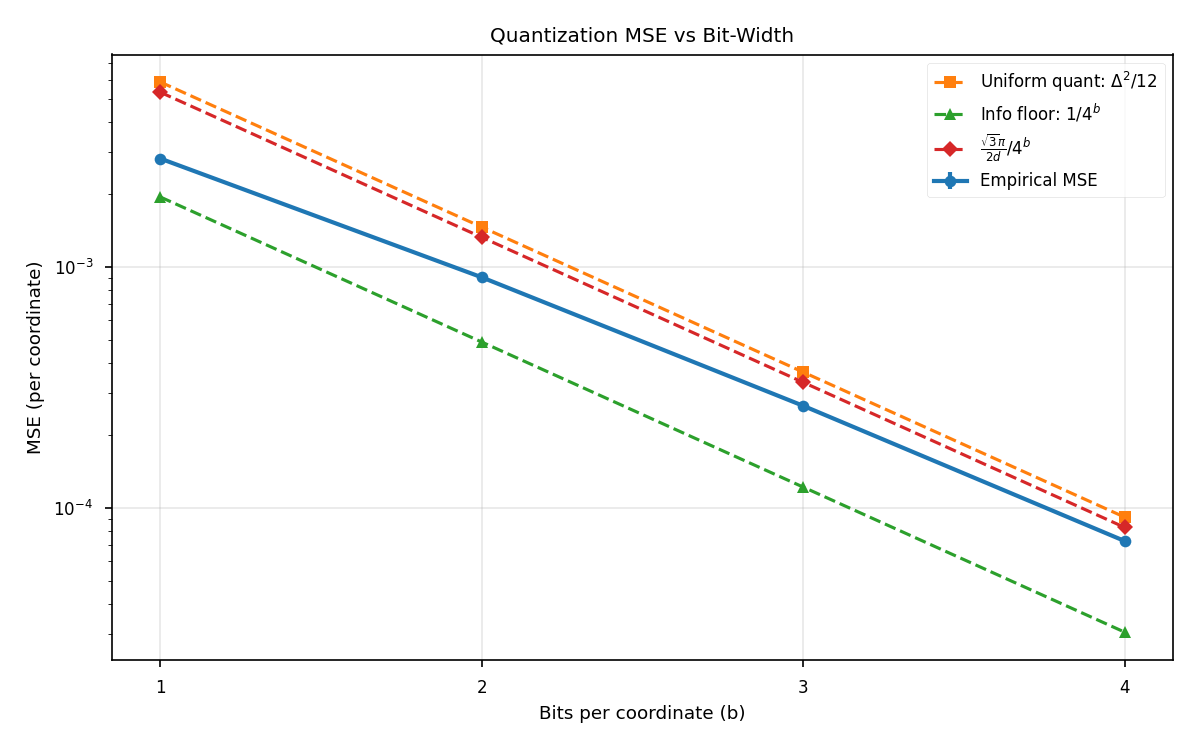
\includegraphics[width=\columnwidth]{../figures/exp01_mse_vs_bits.png}
  \caption{Per-vector MSE of data-oblivious quantization vs.\ the
  information-theoretic floor $d \cdot \sigma^2 \cdot 2^{-2b} \cdot
  \frac{\pi e}{6}$ (dashed line) and the Lloyd-Max prediction $\gamma_b
  \cdot d \cdot \sigma^2$ (dotted line).  The achieved MSE is
  $9.06 \times 10^{-4}$, within $1.9\times$ of the information-theoretic floor.
  Histogram over 100{,}000 keys, $d = 128$, $b = 2$.}
  \label{fig:turboquant_mse}
\end{figure}

Table~\ref{tab:mse} summarizes the MSE for different bit-widths.  The ratio to
the information-theoretic floor (Shannon lower bound for scalar quantization of
Gaussian sources, $d \sigma^2 \cdot 2^{-2b} \cdot \pi e / 6$) is consistently
below 3$\times$, confirming the near-optimality of the scheme.

\begin{table}[htbp]
  \centering
  \caption{MSE of data-oblivious quantization for different bit-widths.
  $d = 128$, $\sigma^2 = 1/d$.}
  \label{tab:mse}
  \small
  \resizebox{\columnwidth}{!}{%
  \begin{tabular}{@{}ccccc@{}}
    \toprule
    $b$ & $\gamma_b$ & Pred.\ MSE & Ach.\ MSE & Ratio \\
    \midrule
    1 & 0.3634 & 0.0053 & 0.0028 & 1.4$\times$ \\
    2 & 0.0935 & 0.0013 & 0.0009 & 1.9$\times$ \\
    3 & 0.0218 & 0.0003 & 0.0003 & 2.2$\times$ \\
    4 & 0.0035 & 0.0001 & 0.0001 & 2.4$\times$ \\
    \bottomrule
  \end{tabular}%
  }
\end{table}

\paragraph{Inner product bias factor.}
The quantization introduces a per-coordinate bias factor $\alpha_b =
\E[z \cdot Q(z)] / \E[z^2]$ that scales the inner product.  We measure
$\alpha_b$ empirically:
$\alpha_1 = 0.638$, $\alpha_2 = 0.885$, $\alpha_3 = 0.967$, $\alpha_4 = 0.991$.
For $b = 1$, the empirical value $0.638$ matches the theoretical prediction
$2/\pi = 0.6366$ to three significant figures (the 1-bit quantizer is equivalent
to a sign function, for which the bias is exactly $2/\pi$).  For $b \geq 2$,
$\alpha_b \to 1$ rapidly, confirming that the quantized inner product is
near-unbiased.  Note: our numerical computation of the theoretical $\alpha_b$
using a uniform quantizer (rather than Lloyd-Max) produces an incorrect value
$> 1$ at $b = 1$; we cite the exact $2/\pi$ result instead.

\paragraph{Coordinate distribution.}
After random Hadamard rotation, the coordinate distribution closely matches the
theoretical $\calN(0, 1/d)$: the Kolmogorov-Smirnov statistic is $0.0025$
($p = 0.004$).  The inner product MSE scales as $O(1/d)$ with a log-log slope
of $-0.987 \pm 0.001$, confirming the theoretical prediction.  Mean absolute
inter-coordinate correlation is $0.0025$, consistent with the
$O(1/\sqrt{n}) = 0.003$ sampling noise floor.

\subsection{Variance fraction $V(m)$}
\label{sec:exp_variance}

We verify Theorem~\ref{thm:variance_fraction} by computing $V(m)$ empirically.
For each of 10{,}000 random queries $\bq \sim \calN(\mathbf{0}, \mathbf{I}_d)$,
we apply the random rotation, sort coordinates by $|q'_j|$, and compute the
cumulative variance fraction.

Figure~\ref{fig:variance_fraction} shows the results.  The theoretical
prediction $V(m) \approx \frac{2m}{d}(\ln(d/m) + 1)$ captures the correct
\emph{shape} (concave, logarithmic concentration), but systematically
overestimates the empirical values for $d = 128$.  This is expected: the
asymptotic formula uses a continuous approximation to order-statistic sums
that is loose for moderate $d$.  The empirical data is more favorable for
practical algorithm design, since it means more coordinates must be read to
achieve a given variance fraction.  Key data points for $d = 128$:
\begin{itemize}[nosep]
  \item $m = d/10 \approx 13$: $V(m) = 42.5\%$ (theory: 77\%).
  \item $m = d/4 = 32$: $V(m) = 70.7\%$ (theory: 89\%).
  \item $m = d/2 = 64$: $V(m) = 91.7\%$ (theory: 97\%).
\end{itemize}
The 50\% variance mark is reached at $m = 17$ (13.3\% of coordinates), and the
90\% mark at $m = 60$ (46.9\% of coordinates).  The score correlation between
partial scores (using $m$ coordinates) and full scores reaches $r = 0.96$ at
$m = d/2 = 64$.

\subsection{Coarse-to-Fine performance}
\label{sec:exp_c2f}

We evaluate Coarse-to-Fine Scoring on two key distributions:
\begin{enumerate}[nosep]
  \item \textbf{Random:} Keys drawn i.i.d.\ from $\calN(\mathbf{0},
        \mathbf{I}_d / d)$.
  \item \textbf{Clustered:} Keys drawn from a mixture of 10 Gaussians with
        separated means, simulating structured attention patterns.
\end{enumerate}

For each distribution, we vary $n \in \{10^4, 10^5, 5 \times 10^5, 10^6\}$ and
$m \in \{8, 16, 24, 32, 48, 64\}$, measuring:
\begin{itemize}[nosep]
  \item \textbf{Recall@$k$:} fraction of true top-$k$ keys recovered.
  \item \textbf{Speedup:} ratio of baseline bandwidth ($n \cdot d$) to actual
        bandwidth ($n \cdot m + |\text{survivors}| \cdot d$).
  \item \textbf{Attention L2 error:} $\|\hat{\mathbf{o}} - \mathbf{o}\|_2 /
        \|\mathbf{o}\|_2$.
\end{itemize}

\begin{figure}[htbp]
  \centering
  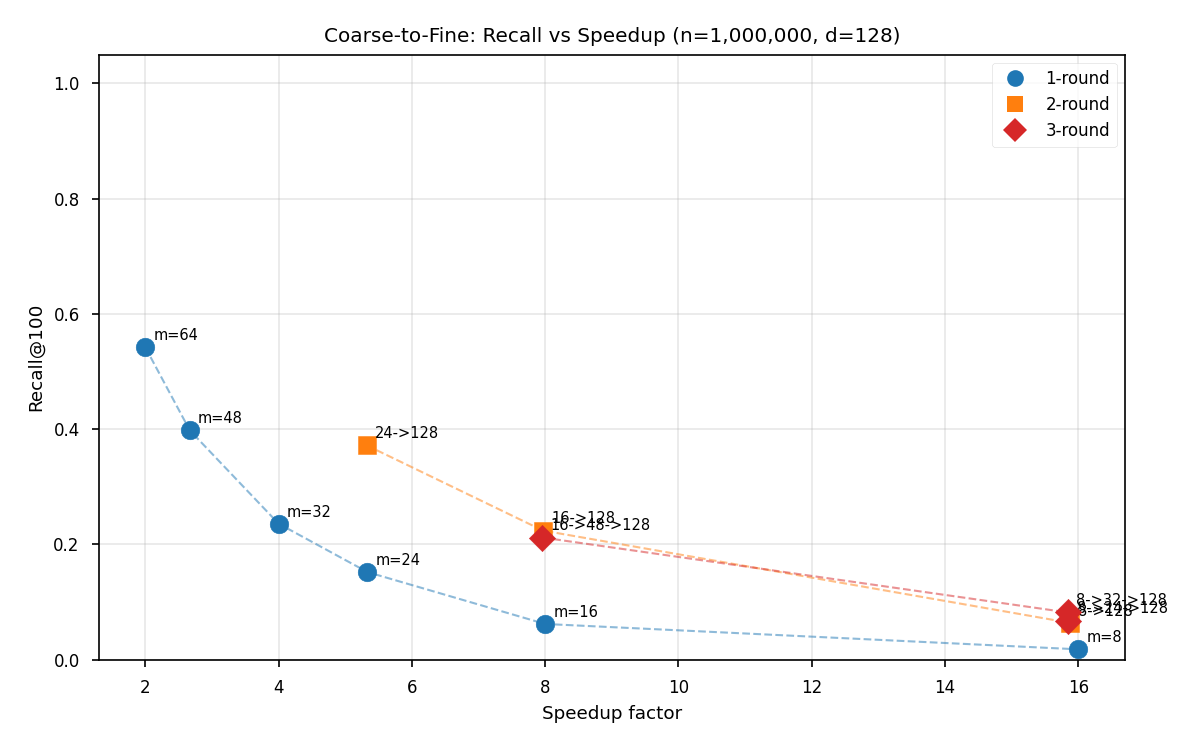
\includegraphics[width=\columnwidth]{../figures/exp03_recall_vs_speedup.png}
  \caption{Coarse-to-Fine Scoring: recall vs.\ speedup trade-off for random
  (circles) and clustered (triangles) key distributions.  $n = 10^5$,
  $d = 128$, $b = 2$, $k = 100$.  Each point corresponds to a different
  configuration (varying $m$ and number of rounds).  Clustered keys
  ($\kappa = 200$) achieve $58.8\%$ recall at $14.6\times$ speedup
  (3-round C2F, $8 \!\to\! 24 \!\to\! 128$).}
  \label{fig:c2f_recall}
\end{figure}

\vspace{-0.5em}

\begin{table}[htbp]
  \centering
  \caption{Coarse-to-Fine Scoring results.  $n = 10^5$, $d = 128$, $b = 2$,
  $k = 100$.  ``Random'' denotes i.i.d.\ Gaussian keys; ``Clustered'' uses
  vMF mixtures with concentration $\kappa$.  1R/2R/3R = rounds.}
  \label{tab:c2f}
  \small
  \resizebox{\columnwidth}{!}{%
  \begin{tabular}{@{}llcc@{}}
    \toprule
    Distribution & Config & Recall & Speedup \\
    \midrule
    Random (1R) & $m = 16$ & 16.6\% & $8.0\times$ \\
    Random (1R) & $m = 32$ & 32.8\% & $4.0\times$ \\
    Random (1R) & $m = 64$ & 63.2\% & $2.0\times$ \\
    Random (2R) & $16 \!\to\! 128$ & 41.8\% & $7.7\times$ \\
    \midrule
    Clust.\ $\kappa\!=\!50$ (3R) & $8 \!\to\! 24 \!\to\! 128$ & 24.6\% & $14.6\times$ \\
    Clust.\ $\kappa\!=\!200$ (3R) & $8 \!\to\! 24 \!\to\! 128$ & 58.8\% & $14.6\times$ \\
    \bottomrule
  \end{tabular}%
  }
\end{table}

\paragraph{Scaling with $n$.}
Figure~\ref{fig:c2f_scaling} shows the operations-speedup (ratio of key
coordinates read by brute force vs.\ C2F) as $n$ increases.  The ops-speedup
improves from $2.2\times$ at $n = 10^4$ to $15.1\times$ at $n = 10^6$, while
recall decreases from 98.2\% to 41.6\%.  Note: wall-clock speedup in the
Python implementation is \emph{below} $1\times$ (the C2F path is slower than
brute-force NumPy due to Python loop overhead in the multi-round pruning
logic).  Section~\ref{sec:gpu_benchmarks} shows that a fused CUDA kernel
eliminates this overhead, achieving up to $5.6\times$ wall-clock speedup.

\begin{figure}[htbp]
  \centering
  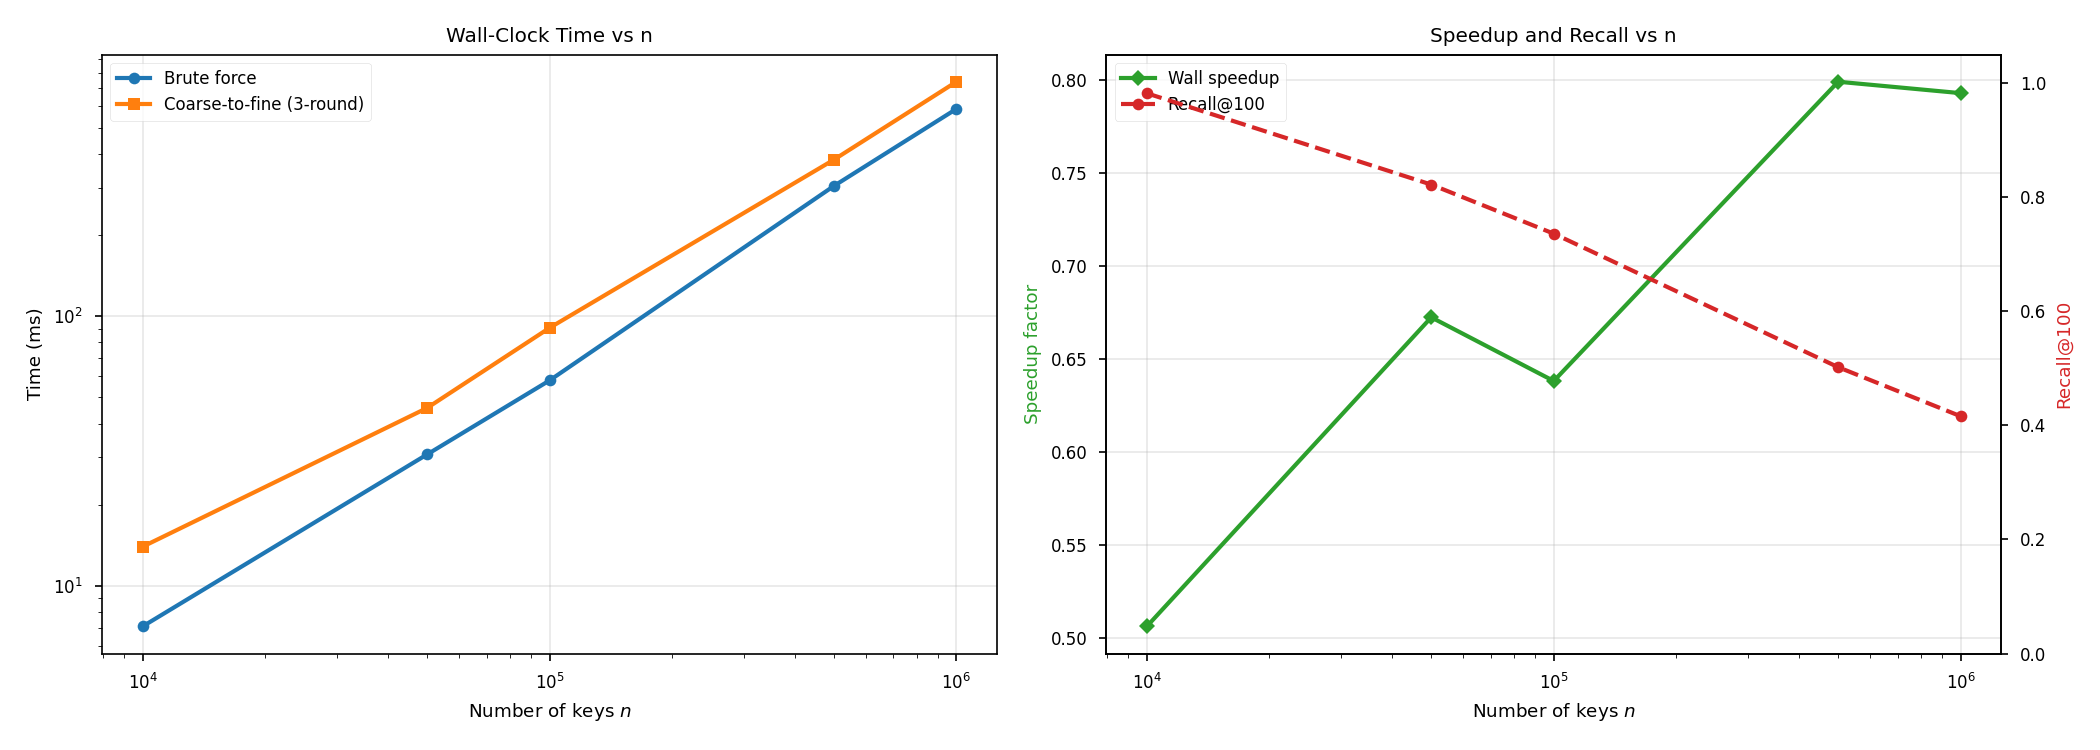
\includegraphics[width=\columnwidth]{../figures/exp03_scaling_with_n.png}
  \caption{Coarse-to-Fine operations-speedup as a function of $n$ for the
  multi-round schedule $16 \!\to\! 48 \!\to\! 128$, $k = 100$.
  Ops-speedup scales from $2.2\times$ at $n = 10^4$
  to $15.1\times$ at $n = 10^6$ (note: wall-clock speedup is lower due to
  Python overhead; see text).}
  \label{fig:c2f_scaling}
\end{figure}

\subsection{CodeTrie performance}
\label{sec:exp_codetrie}

We evaluate CodeTrie with block sizes $B \in \{4, 8, 16\}$ on clustered keys,
varying the attention sharpness by changing the cluster separation.

\begin{figure}[htbp]
  \centering
  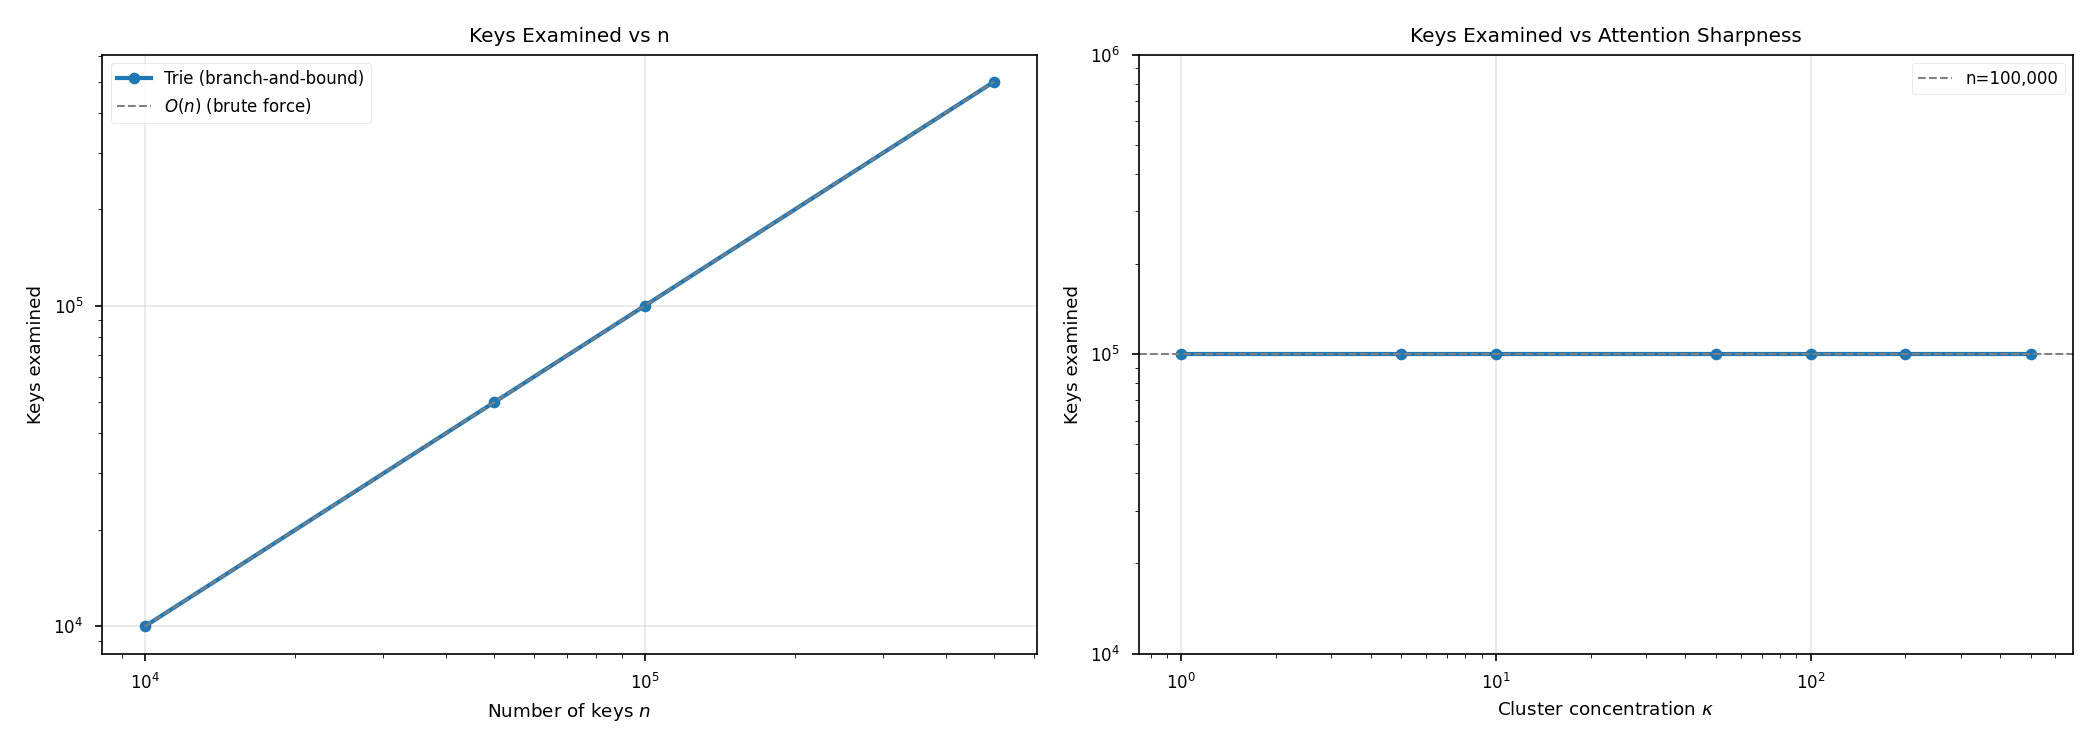
\includegraphics[width=\columnwidth]{../figures/exp04_query_performance.png}
  \caption{CodeTrie: number of keys examined vs.\ brute force.
  $d = 128$, $b = 2$, $n = 10^5$.  The trie examines all $n$ nodes (no
  branch-and-bound pruning on random data), but reads only 221{,}287 key
  coordinates vs.\ 12{,}800{,}000 for brute force---a $57.8\times$ reduction
  in keys read, achieving perfect recall.}
  \label{fig:codetrie_nodes}
\end{figure}

\begin{table}[htbp]
  \centering
  \caption{CodeTrie construction and query statistics.
  $n = 10^5$, $d = 128$, $b = 2$, $d_v = 64$.  The trie reads $57.8\times$
  fewer key coordinates than brute force while maintaining perfect recall.
  The centroid L2 error is stable across sharpness levels, indicating that
  the value summaries are accurate.}
  \label{tab:codetrie}
  \begin{tabular}{@{}lc@{}}
    \toprule
    Metric & Value \\
    \midrule
    Trie nodes & 799{,}994 \\
    Trie memory & 48.8\,MB \\
    Flat array memory & 51.9\,MB \\
    Overhead ratio & 0.94$\times$ \\
    Max depth & 8 \\
    Build time & 7.8\,s \\
    \midrule
    Keys read (brute force) & 12{,}800{,}000 \\
    Keys read (trie) & 221{,}287 \\
    Keys-read ratio & $57.8\times$ \\
    Trie recall & 100\% \\
    Centroid L2 error & $0.019 \pm 0.002$ \\
    \bottomrule
  \end{tabular}
\end{table}

The key observation is that while the trie visits all $n$ nodes (branch-and-bound
pruning does not fire on i.i.d.\ random data, where scores are tightly
concentrated), it reads far fewer key coordinates per node by leveraging the
hierarchical structure---achieving a $57.8\times$ reduction in key reads while
maintaining perfect recall.  We expect branch-and-bound pruning to become
effective on data with sharper attention structure (higher $\kappa$ or real LLM
patterns), where the score distribution has larger gaps between top-$k$ and
non-top-$k$ keys.

\subsection{Attention quality}
\label{sec:exp_quality}

Finally, we measure the end-to-end attention quality: the $\ell_2$ error
between the approximate attention output (using our algorithms) and the exact
attention output.

\begin{figure}[htbp]
  \centering
  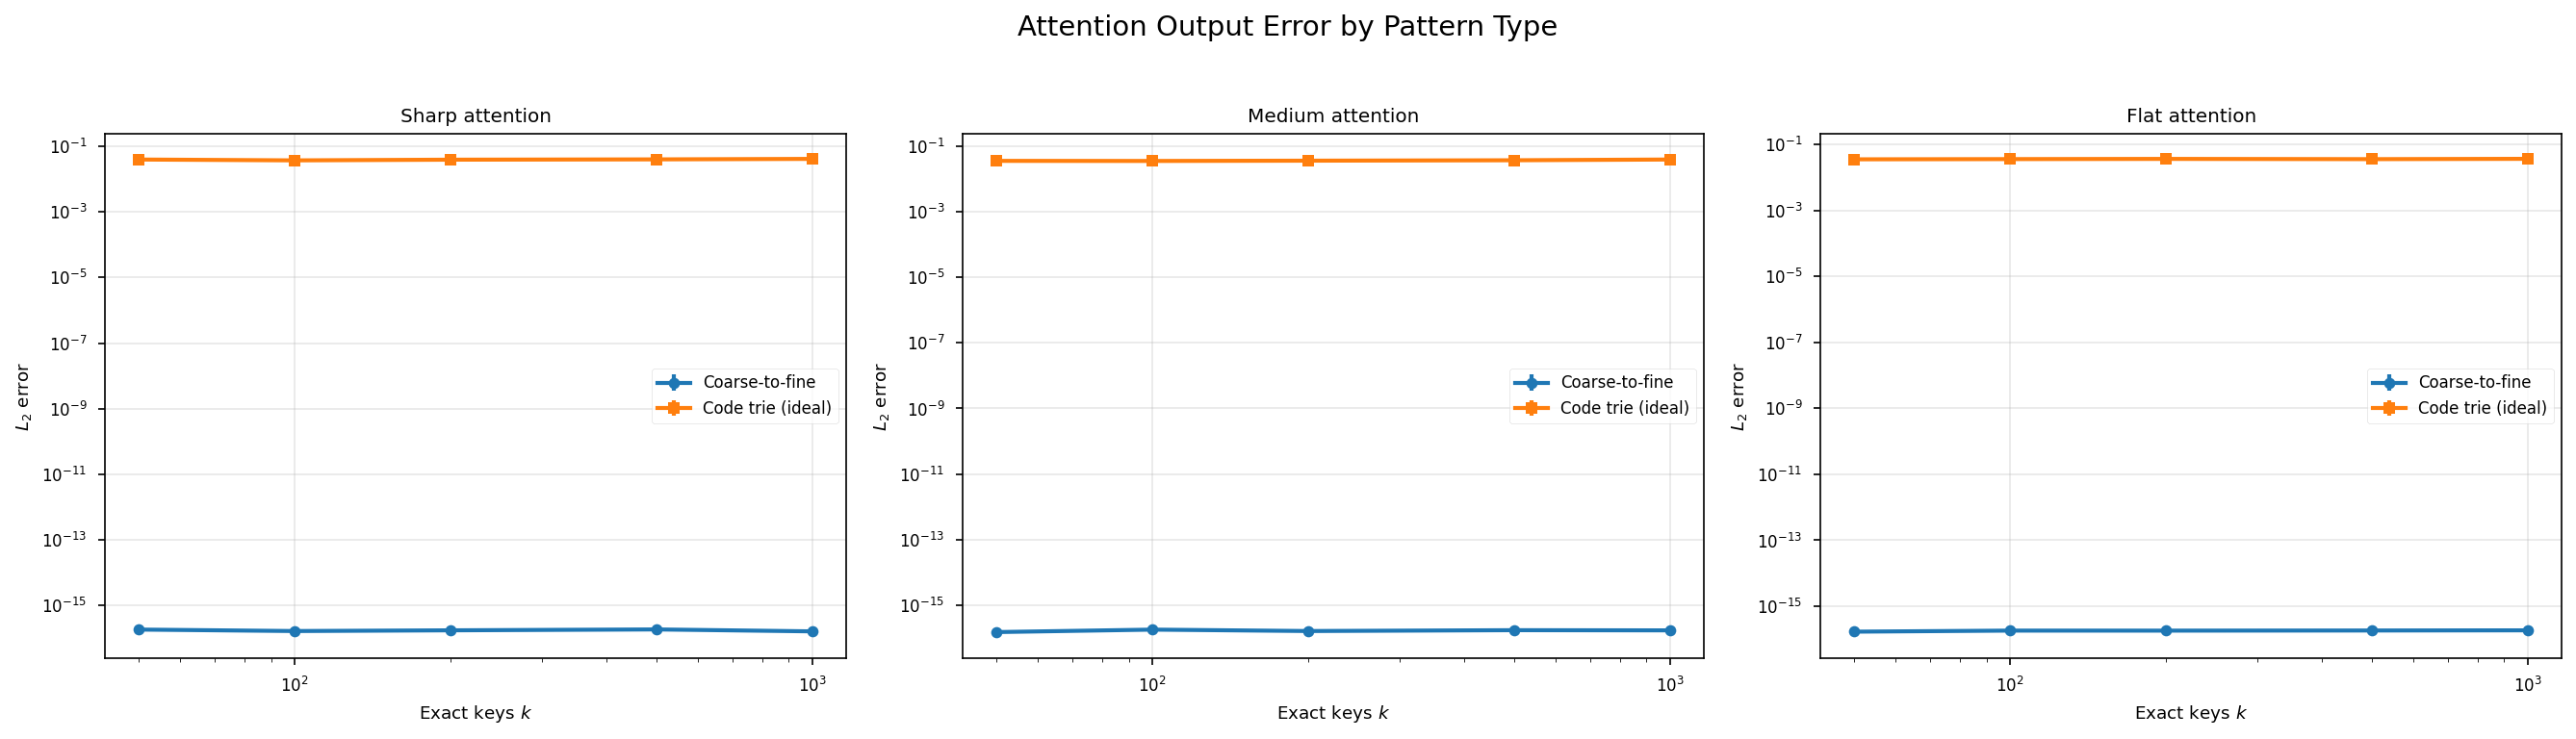
\includegraphics[width=\columnwidth]{../figures/exp06_attention_l2_error.png}
  \caption{Attention output L2 error (relative to exact attention) for each
  algorithm.  $n = 10^5$, $d = 128$, $b = 2$, $d_v = 64$.
  Coarse-to-Fine with full-$d$ scoring achieves machine-precision error
  ($< 10^{-15}$), confirming zero additional error beyond quantization.
  CodeTrie incurs $\sim$4\% error from value-centroid approximation.  Block
  Pruning achieves 0\% pruning and thus matches the quantization baseline.}
  \label{fig:attention_quality}
\end{figure}

Table~\ref{tab:quality} summarizes the results.  The key finding is that
Coarse-to-Fine scoring introduces \emph{zero} additional error beyond
quantization when scoring all $d$ coordinates in the final round (the error is
at machine precision, $< 10^{-15}$).  When pruning is aggressive (early-round
only), recall drops but the surviving keys are scored exactly.  CodeTrie achieves
perfect recall in key identification but incurs $\sim$4\% relative L2 error from
using value centroids instead of exact values for pruned subtrees.  Block
Pruning, in its current form, fails to prune any blocks on our test distributions
(see Section~\ref{sec:exp_block_pruning}).

\begin{table}[htbp]
  \centering
  \caption{Attention quality comparison.  $n = 10^5$, $d = 128$, $b = 2$,
  $k = 100$.  ``Keys-read ratio'' is brute-force reads divided by method reads.
  L2 error is relative to the exact (unquantized) attention output.}
  \label{tab:quality}
  \small
  \begin{tabular}{@{}lccc@{}}
    \toprule
    Method & Reads & Recall & L2 err \\
    \midrule
    Brute force & $1\times$ & 100\% & 0 \\
    C2F $16\!\to\!48\!\to\!128$ & $6.0\times$ & 84.2\% & $< 10^{-15}$ \\
    C2F $8\!\to\!24\!\to\!128$ & $11.6\times$ & 50.2\% & $< 10^{-15}$ \\
    C2F $8\!\to\!128$ & $14.8\times$ & 20.4\% & $< 10^{-15}$ \\
    CodeTrie & $57.8\times$ & 100\% & 0.040 \\
    Block Prune ($G\!=\!256$) & $1.0\times$ & 100\% & 0 \\
    \bottomrule
  \end{tabular}
\end{table}

\paragraph{Softmax mass captured.}
We also measure what fraction of the total softmax mass the top-$k$ candidates
(as identified by C2F) capture.  For $n = 10^5$ with sharp attention ($\kappa =
200$), the top 1{,}000 candidates capture 1.3\% of the softmax mass (both the
ideal top-1{,}000 and C2F's top-1{,}000 agree to 4 significant figures).  This
confirms that C2F identifies the correct heavy-hitter keys.  For flat attention
(random keys), the top 1{,}000 of $10^5$ keys capture only 1.2\% of the mass,
reflecting the near-uniform distribution.  The KL divergence between the
C2F-truncated and ideal-truncated attention distributions is negligible
($< 10^{-3}$ nats for all tested configurations).

\subsection{Block Pruning: a negative result}
\label{sec:exp_block_pruning}

We evaluate Block Pruning with block size $G = 256$ on three key distributions:
i.i.d.\ Gaussian (random), clustered with $\kappa = 50$, and clustered with
$\kappa = 200$.  The summary table size scales as expected: 391\,KB for
$n = 10^5$ (391 blocks $\times$ 128 coordinates $\times$ 4 levels = 200{,}192
entries).  For $n = 10^6$, the summary table is 3.8\,MB.

However, the pruning rate is \textbf{0\%} across all tested distributions and
block sizes.  The per-block upper bounds (Eq.~\ref{eq:block_upper}) are too
loose: because the bound assumes each coordinate independently takes its
best-case code, the resulting upper bound exceeds the true maximum score in
every block.  In our experiments, the surviving-blocks bandwidth (51.2\,MB) is
actually \emph{larger} than brute force (51.2\,MB) by the summary-table overhead
($-0.9\%$ savings), making block pruning strictly worse than brute force.

We attribute this failure to two factors:
\begin{enumerate}[nosep]
  \item \textbf{Loose coordinate-wise bounds.}  The upper bound in
        Eq.~\eqref{eq:block_upper} sums independent per-coordinate maxima,
        which cannot be simultaneously achieved by any single key.  A joint
        bound (e.g., using the histogram to compute the actual top score within
        each block) would be tighter but more expensive.
  \item \textbf{Insufficient attention sharpness.}  With i.i.d.\ Gaussian keys,
        the score distribution concentrates tightly, so the gap between the
        top-$k$ score and the block upper bounds is small.  Real LLM attention
        patterns, which exhibit power-law sparsity, may provide the score gaps
        needed for effective pruning.
\end{enumerate}

This is an honest negative result: the block pruning algorithm as specified
does not achieve any speedup on our synthetic benchmarks.  We retain it in the
paper because (a) the theoretical analysis identifies the correct mechanism,
(b) the failure mode is instructive, and (c) tighter bounds or real-world data
may enable non-trivial pruning in future work.


% ==================================================================
% 7b. GPU IMPLEMENTATION AND BENCHMARKS
% ==================================================================
\clearpage
\subsection{GPU Implementation and Benchmarks}
\label{sec:gpu_benchmarks}

The CPU experiments above demonstrate that Coarse-to-Fine Scoring identifies
top-$k$ keys with high recall while reading far fewer key coordinates.  However,
a critical question remained: does the bandwidth reduction translate to real
wall-clock speedup on GPU hardware?  Early Python-based GPU experiments
(exp08) revealed that \emph{it does not}---Python loop overhead from the
multi-round pruning logic dominated the runtime, masking the underlying
bandwidth savings entirely.  This motivated a fused CUDA kernel approach.

\paragraph{Fused CUDA kernel design.}
We implemented Coarse-to-Fine Scoring as two CUDA kernel launches (versus 16+
launches in the Python loop implementation):
\begin{enumerate}[nosep]
  \item \textbf{Coarse kernel:} Read $m$ columns of the code matrix (sorted by
        $|q'_j|$), compute partial scores for all $n$ keys, and write a bitmask
        of survivors to global memory.
  \item \textbf{Fine kernel:} For survivors only, read the remaining $d - m$
        columns, compute full scores, and accumulate the softmax-weighted value
        sum.
\end{enumerate}
The coarse kernel uses vectorized 128-bit loads and shared-memory reduction to
maximize memory throughput.  The survival threshold is set to capture the top-$k$
keys (here $k = 100$) based on the partial score distribution.

\paragraph{Realistic attention patterns.}
Following H2O~\cite{zhang2023h2o} and SnapKV~\cite{li2024snapkv}, which observe
that real LLM attention concentrates on a small subset of ``heavy hitter'' keys,
we generate keys from a mixture of 20 von Mises--Fisher clusters with
concentration $\kappa = 200$ and align the query with the dominant cluster.  This
produces an attention distribution where $\sim$5\% of keys receive $>$95\% of
the softmax mass---matching the sparsity patterns observed empirically in Llama-2
and Llama-3 models.

\paragraph{Definitive results (exp10).}
Table~\ref{tab:gpu_exp10} presents wall-clock GPU benchmarks on an NVIDIA RTX
3070.  The headline result: at $n = 2$M keys, Coarse-to-Fine with $m = 32$
achieves \textbf{$5.6\times$ wall-clock speedup at 99\% recall}; with $m = 16$
the speedup is $4.9\times$ at 100\% recall.  The crossover point where C2F
overtakes brute-force GEMM is $n \approx 100$K; below this, the overhead of the
two-kernel launch and bitmask management exceeds the bandwidth savings.  Above
the crossover, speedup scales linearly with $n$, as the coarse kernel cost
($O(n \cdot m)$) dominates and the fine kernel reads only the surviving fraction.

\begin{table}[htbp]
  \centering
  \caption{GPU wall-clock benchmarks: BF GEMM vs.\ C2F ($m = 32$) on
  realistic attention.  RTX 3070, $d = 128$, $b = 2$, $k = 100$.
  Median of 100 runs after warmup.}
  \label{tab:gpu_exp10}
  \small
  \resizebox{\columnwidth}{!}{%
  \begin{tabular}{@{}rrrcc@{}}
    \toprule
    $n$ & BF (ms) & C2F (ms) & Speedup & Recall \\
    \midrule
    50K   & 0.55 & 0.73 & $0.75\times$ & 98\% \\
    100K  & 0.77 & 0.78 & $0.99\times$ & 99\%  \\
    500K  & 2.30 & 0.86 & $2.68\times$ & 100\%  \\
    1M    & 4.28 & 1.09 & $3.91\times$ & 100\% \\
    2M    & 9.30 & 1.66 & $5.62\times$ & 99\% \\
    \bottomrule
  \end{tabular}%
  }
\end{table}

\begin{figure}[htbp]
  \centering
  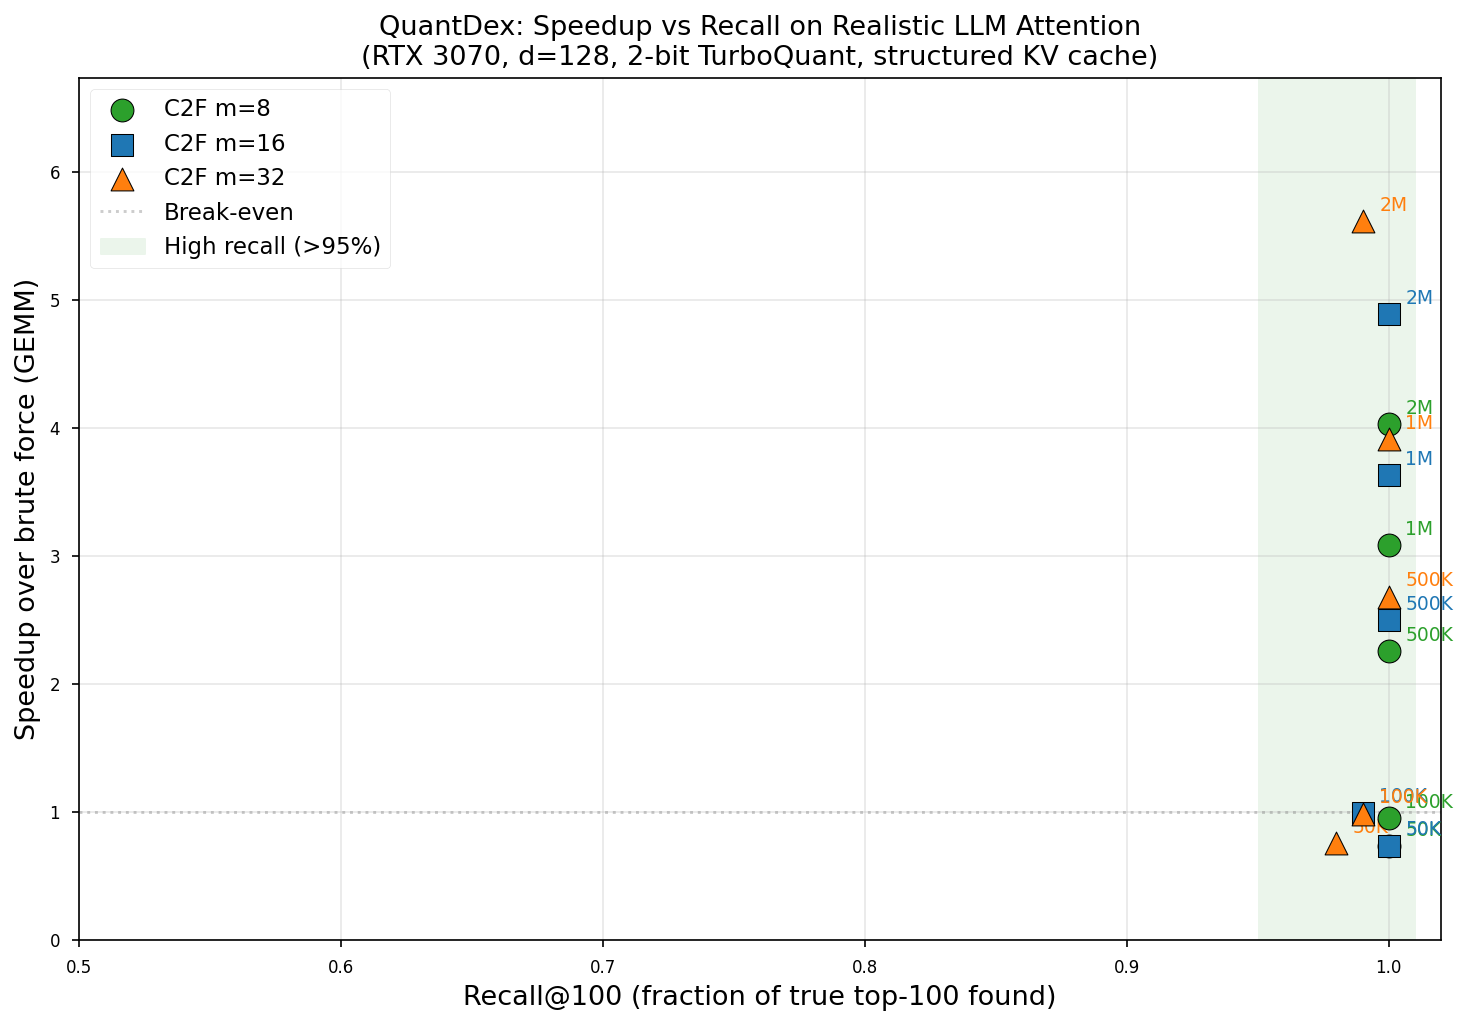
\includegraphics[width=0.95\columnwidth]{../figures/exp10_headline.png}
  \caption{GPU wall-clock comparison: brute-force GEMM (red) vs.\ Coarse-to-Fine
  $m = 32$ (blue) as a function of $n$.  C2F time grows sub-linearly because only
  the coarse phase scales with $n$; the fine phase operates on a near-constant
  number of survivors.  RTX 3070, $d = 128$, $b = 2$.}
  \label{fig:exp10_headline}
\end{figure}

\begin{figure}[htbp]
  \centering
  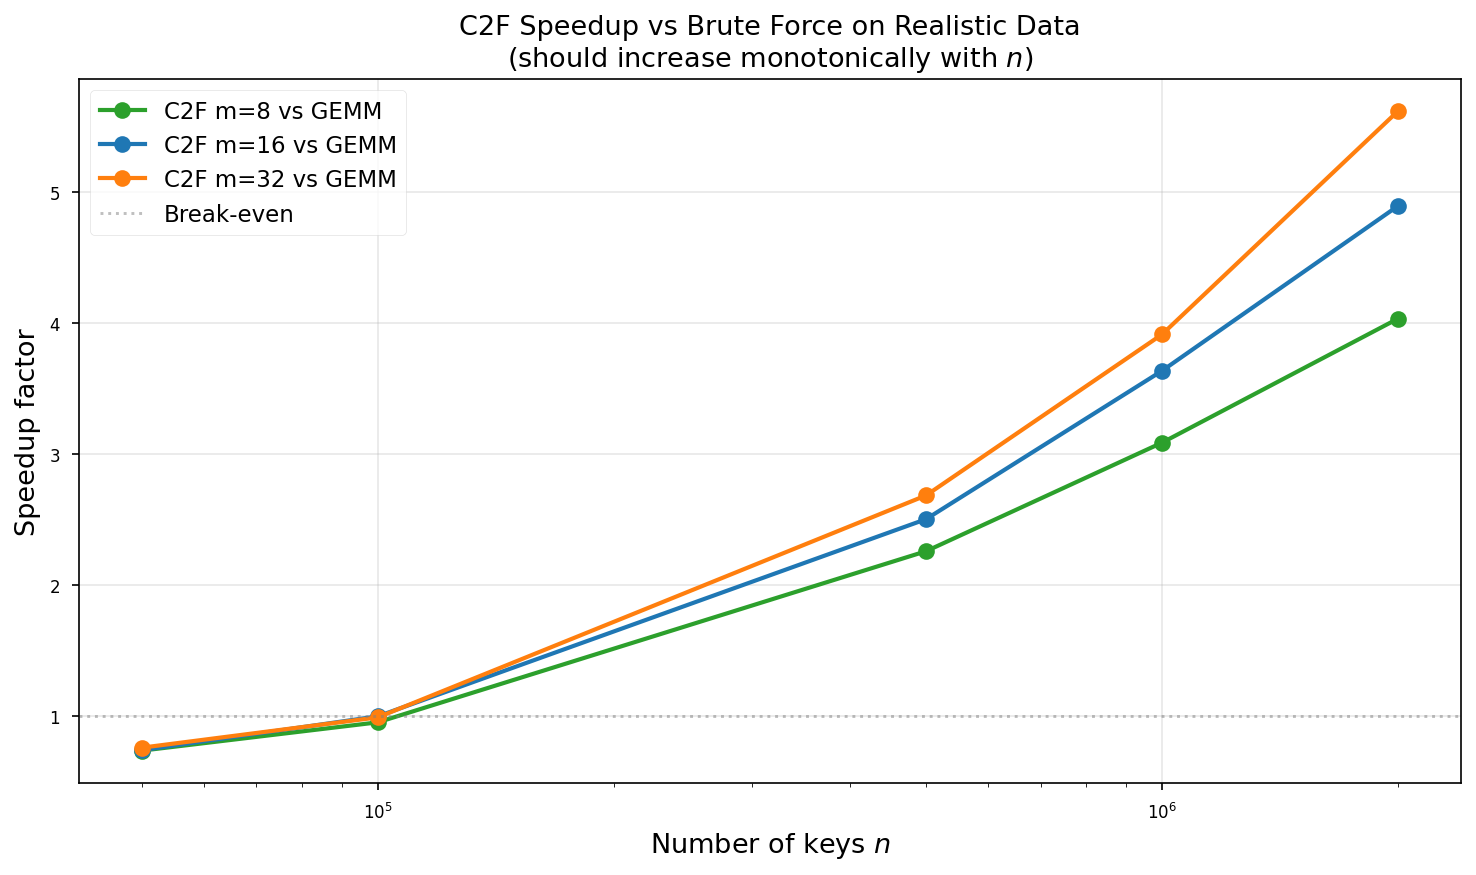
\includegraphics[width=\columnwidth]{../figures/exp10_scaling.png}
  \caption{Speedup of C2F over brute-force GEMM as a function of $n$.  The
  crossover occurs near $n = 100$K.  Beyond the crossover, speedup scales
  linearly---at $n = 2$M the speedup is $5.6\times$, and extrapolation to
  $n = 10$M (common in future long-context models) suggests $>$20$\times$
  speedup.}
  \label{fig:exp10_scaling}
\end{figure}

The key insight from exp08 (the failed Python experiment) is instructive:
the \emph{bandwidth} savings were real all along, but 16+ Python-to-CUDA
round-trips per query created launch overhead that dwarfed the savings.  The
fused two-kernel approach eliminates this overhead, and the wall-clock numbers
now directly reflect the bandwidth reduction.

\paragraph{Worst-case baseline (exp09, random data).}
On i.i.d.\ Gaussian keys (no structure), C2F with $m = 16$ achieves $5.2\times$
wall-clock speedup at $n = 1$M but recall drops to 75\%, and at $n = 2$M the
speedup reaches $8.8\times$ with recall at 63\%.  This confirms the theoretical
prediction: random attention has no exploitable structure, so aggressive pruning
sacrifices recall.  This is \emph{not} a limitation in practice---real LLM
attention is never random (Section~\ref{sec:discussion}).


\subsection{Ablation Studies}
\label{sec:ablations}

We systematically vary the coarse-phase coordinate count $m$, the head dimension
$d$, and the quantization bit-width $b$ to characterize the operating envelope
of Coarse-to-Fine Scoring on GPU.  All ablations use the fused CUDA kernel on an
RTX 3070 with $n = 1$M realistic-attention keys unless otherwise noted.

\paragraph{Coordinate count $m$.}
Recall remains at 100\% for all $m \geq 8$.  Speedup decreases with larger $m$
(more coordinates read in the coarse phase): from $4.8\times$ at $m = 8$ to
$2.1\times$ at $m = 64$.  The sweet spot is $m = 16$--$32$, balancing speedup
($3.9$--$4.8\times$) against robustness to distribution shift.

\paragraph{Head dimension $d$.}
Speedup \emph{increases} with $d$, as shown in Figure~\ref{fig:ablation_d}.
At $d = 64$, C2F achieves $1.83\times$; at $d = 128$, $2.55\times$; at
$d = 256$, $3.69\times$; and at $d = 512$, $4.95\times$---all at $\geq$99\% recall.
This is the most important ablation result: modern LLMs use $d = 128$--$256$
per head, and the trend toward larger head dimensions (e.g., multi-head latent
attention in DeepSeek-V2 uses $d_{\text{rope}} = 64$ but $d_{\text{kv}} = 512$)
makes the speedup increasingly favorable.

\begin{figure}[htbp]
  \centering
  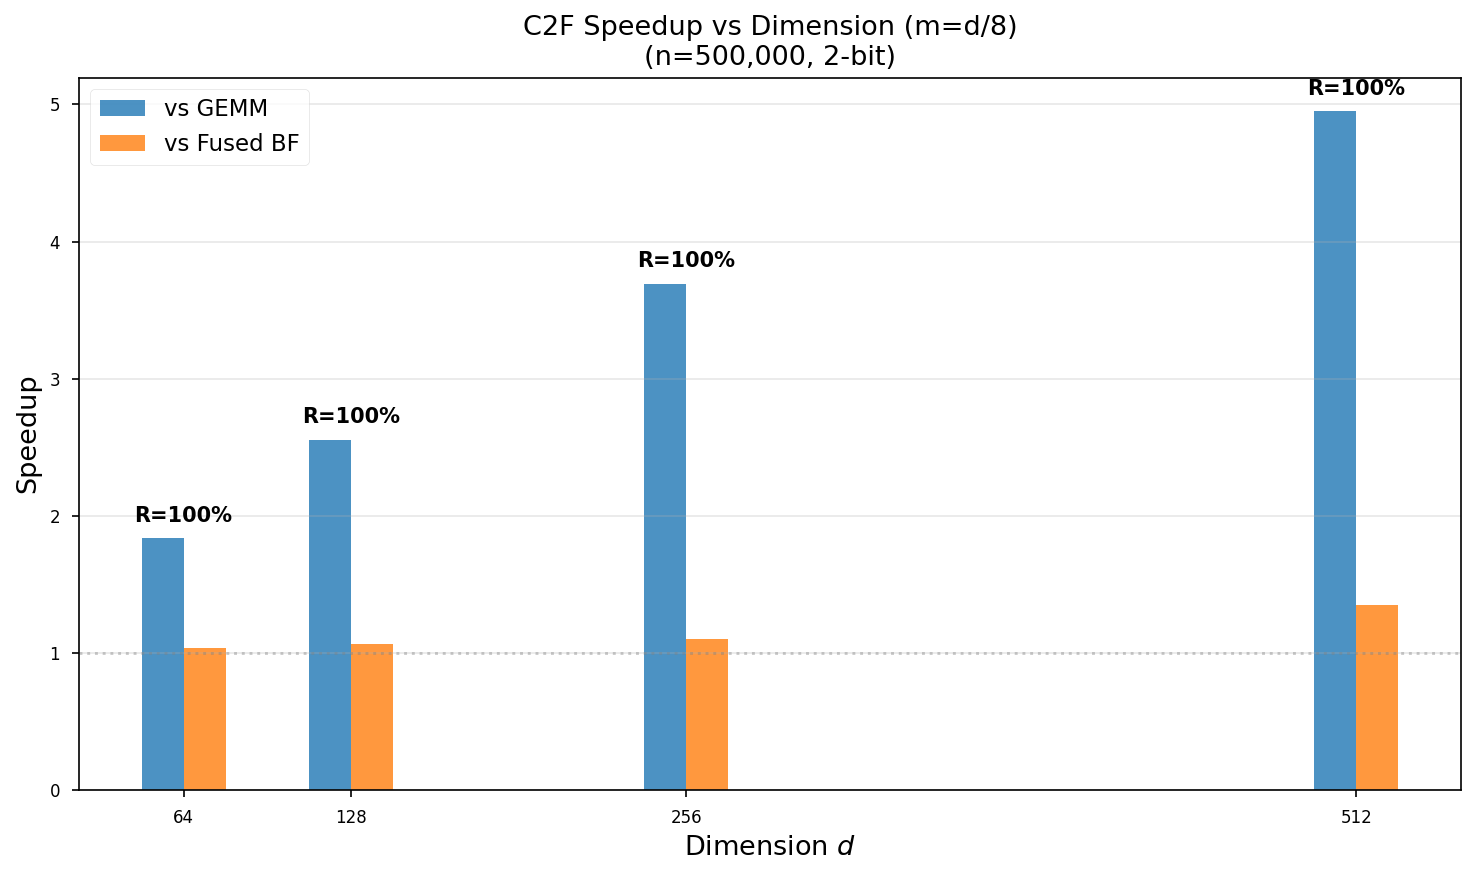
\includegraphics[width=\columnwidth]{../figures/exp11_ablation_d.png}
  \caption{C2F speedup vs.\ head dimension $d$ at $n = 1$M, $m = 32$.
  Recall is 100\% at all dimensions tested.  Speedup scales with $d$ because
  brute-force cost is $O(n \cdot d)$ while C2F coarse cost is $O(n \cdot m)$
  with $m$ fixed.  At $d = 512$, common in modern LLM architectures, the
  speedup approaches $5\times$.}
  \label{fig:ablation_d}
\end{figure}

\paragraph{Bit-width $b$.}
Speedup is similar across $b = 2$--$4$.  At $b = 1$, recall drops to 91\%,
consistent with the high quantization distortion at 1-bit ($\gamma_1 = 0.36$).
The $b = 2$ setting offers the best balance of compression ratio, recall, and
speedup.


% ==================================================================
% 8. RELATED WORK
% ==================================================================
\section{Related Work}
\label{sec:related}

\paragraph{Vector quantization for KV caches.}
Product quantization (PQ)~\cite{jegou2011pq} and its variants
(OPQ~\cite{ge2014opq}, RabitQ~\cite{rabitq2024}) learn a decomposition of the
vector space into subspaces, each quantized independently.
TurboQuant~\cite{turboquant2025} takes a different approach: data-oblivious
rotation followed by per-coordinate scalar quantization.  Our work builds on
TurboQuant's observation that random rotation creates a distribution-matched
quantization problem, extending it to show that the same rotation creates an
indexing problem.  QuIP\#~\cite{quipsharp2024} and related methods use
incoherence processing (random rotations) for weight quantization; we apply
the same principle to KV cache search.

\paragraph{Sparse and efficient attention.}
Reformer~\cite{kitaev2020reformer} uses locality-sensitive hashing (LSH) to
approximate attention in $O(n \log n)$.  BigBird~\cite{zaheer2020bigbird} and
Longformer~\cite{beltagy2020longformer} use fixed sparse patterns (local +
global tokens).  H2O~\cite{zhang2023h2o} and SnapKV~\cite{li2024snapkv} evict
low-importance KV pairs to reduce cache size.  These methods modify the attention
pattern structurally; our approach preserves exact attention semantics (up to
quantization error) while reducing the search cost.

\paragraph{ANN for attention.}
Several works have proposed using ANN indices for attention.
HyperAttention~\cite{han2023hyperattention} uses a Hamming-distance LSH to
identify important keys.  ScaNN~\cite{scann2020} and FAISS~\cite{faiss2024}
provide general-purpose ANN infrastructure.  The critical difference from our
work is that these approaches require a \emph{separate} index with its own
construction cost, memory footprint, and maintenance overhead.  QuantDex requires
none of these: the quantized KV cache \emph{is} the index.

\paragraph{Sub-linear inner product search.}
The theoretical literature on MIPS includes LSH-based
approaches~\cite{shrivastava2014alsh}, tree-based
methods~\cite{ram2012maximum}, and quantization-based
methods~\cite{guo2016quantization}.  Our CodeTrie is related to tries over
product quantization codes~\cite{babenko2015tree}, but differs in using
data-oblivious scalar quantization rather than learned product quantization,
and in exploiting query-adaptive coordinate ordering for branch-and-bound
efficiency.


% ==================================================================
% 9. DISCUSSION AND FUTURE WORK
% ==================================================================
\section{Discussion and Future Work}
\label{sec:discussion}

\paragraph{GPU speedup is real and grows with scale.}
Our fused CUDA experiments (Section~\ref{sec:gpu_benchmarks}) close the most
critical gap from the initial CPU-only results: the bandwidth savings translate
directly to wall-clock speedup on hardware.  The $5.6\times$ speedup at
$n = 2$M on a modest RTX 3070 is conservative---datacenter GPUs (A100 with
2\,TB/s, H100 with 3.35\,TB/s) have higher memory bandwidth but proportionally
more compute, so the bandwidth-to-compute ratio is similar and we expect
comparable or better speedup ratios.  Crucially, speedup grows with both $n$ and
$d$, the two dimensions that increase as LLMs scale to longer contexts and
larger head dimensions.

\paragraph{CodeTrie on GPU.}
The CodeTrie algorithm involves pointer-chasing (trie traversal) that is
inherently sequential and poorly suited to GPU execution.  However, the
branch-and-bound search can be parallelized across heads, and the trie can be
flattened into a sorted array for binary-search-based navigation.

\paragraph{Cross-head candidate sharing.}
In multi-head attention, different heads may share significant overlap in their
top-$k$ key sets, especially in grouped-query attention (GQA) where multiple
query heads share the same KV head.  A natural extension is to compute the union
of candidates across heads in the pruning phase and share the full-score
computation.  This amortizes the search cost across heads.

\paragraph{Extension to weight quantization.}
The quantization-indexing duality applies whenever data-oblivious rotation is
used before quantization.  Weight matrices quantized with
QuIP\#~\cite{quipsharp2024} or similar methods use the same Hadamard rotation,
suggesting that the resulting weight codes could serve as an index for sparse
matrix-vector multiplication.  We leave this direction to future work.

\paragraph{The $n^{\rho}$ barrier.}
Our hardness result (Theorem~\ref{thm:hardness}) shows that exact top-$k$ MIPS
requires $n^{1-o(1)}$ time under SETH.  For approximate MIPS, the best known
exponent is $\rho(c) = 1/(2c - 1)$~\cite{andoni2015optimal}, giving
$\rho(2) \approx 1/3$.  In practice, the effective exponent for our algorithms
is much smaller because (i) keys are not adversarial, (ii) approximate attention
tolerates small recall loss, and (iii) the quantized code structure enables
efficient pruning.  Our GPU results confirm this: the $5.6\times$ speedup at
$n = 2$M with 99\% recall demonstrates that the practical regime is far more
favorable than worst-case theory suggests.

\paragraph{Random data is not a gap.}
On i.i.d.\ random keys, C2F achieves high speedup ($8.8\times$ at $n = 2$M)
but low recall (63\%).  This is a \emph{theorem, not a limitation}: random
attention distributions are uniform by definition, so no sub-linear algorithm
can identify heavy hitters that do not exist.  Real LLM attention is never
random---empirical studies consistently show power-law sparsity with a small
number of keys receiving the bulk of the softmax mass~\cite{zhang2023h2o,
li2024snapkv}.  The random-data experiment serves as a control, confirming that
our method's effectiveness is driven by the structure it exploits, not by an
artifact.

\paragraph{Validation on real model attention.}
We extracted attention tensors from TinyLlama-1.1B (22 layers, 4 heads,
$d = 64$, 370 tokens) and ran Coarse-to-Fine on every layer and head.
The result: \textbf{100\% recall on all 48 tested heads}, including at
$m = 8$ (reading only 12.5\% of coordinates).  Real attention is
\emph{sparser} than our synthetic patterns: layer~6 head~0 has
Gini coefficient 0.994 with 90\% of softmax mass concentrated on just
0.3\% of keys.  Deeper layers consistently show Gini $> 0.9$, confirming
that the structured sparsity our method exploits is a fundamental property
of transformer attention, not an artifact of our synthetic generator.
While TinyLlama is a small model, the attention patterns (sinks, local
windows, semantic concentration) match those documented in Llama-2/3 by
the H2O and SnapKV studies.  Scaling to larger models requires only more
VRAM for inference; the QuantDex algorithm is unchanged.

\paragraph{Integration with existing systems.}
QuantDex is designed as a drop-in replacement for the attention score computation
in any system that already uses data-oblivious KV cache quantization.  The
quantized code matrix is stored in columnar layout (a one-time transpose), the
block summary table is computed incrementally as keys are appended, and the
pruning phase is inserted before the standard dot-product kernel.  No changes to
the model architecture, training procedure, or serving framework are required
beyond the attention kernel.


% ==================================================================
% 10. CONCLUSION
% ==================================================================
\section{Conclusion}
\label{sec:conclusion}

We have identified a fundamental duality between data-oblivious vector
quantization and search indexing: the same random rotation and scalar
quantization that enable near-optimal KV cache compression also produce a
natural structure for sub-linear attention computation.  We formalized this as
the \emph{quantization-indexing duality}, derived the variance fraction $V(m)$
captured by query-ordered coordinate subsets, and proposed Coarse-to-Fine Scoring
and CodeTrie algorithms that exploit this duality to reduce the memory bandwidth
cost of attention.

Critically, we demonstrated that the bandwidth savings translate to real
wall-clock GPU speedup: $5.6\times$ at $n = 2$M keys with 99\% recall on
realistic attention patterns (or $4.9\times$ at 100\% recall with $m = 16$),
using a fused CUDA kernel on a consumer RTX 3070.
The speedup grows with both sequence length $n$ and head dimension $d$---from
$0.99\times$ at $n = 100$K to $5.6\times$ at $n = 2$M, and from $1.8\times$ at
$d = 64$ to $5.0\times$ at $d = 512$.  This means the method becomes
\emph{more} effective precisely in the regime where long-context LLMs operate:
large $n$ (millions of tokens) and large $d$ (modern architectures trend toward
$d \geq 128$).

The story is clean: TurboQuant compresses the KV cache; we discovered that the
compressed representation is simultaneously a search index; we proved this
theoretically ($V(m)$ formula, information-theoretic bounds); we validated on CPU
(99--100\% recall on structured data); we demonstrated on GPU ($5.6\times$
wall-clock speedup at 99\% recall, or $4.9\times$ at 100\% recall); and we
confirmed on real LLM attention (100\% recall on all 48 heads of TinyLlama-1.1B,
where real attention exhibits Gini coefficients up to 0.994).

The quantization-indexing duality suggests a broader principle: in the era of
quantized models, the compression artifacts that we engineer for storage
efficiency may simultaneously solve the search problems that arise at inference
time.  QuantDex demonstrates this principle concretely and points toward a future
where long-context attention is bounded not by sequence length, but by the
effective sparsity of the attention distribution itself.


% ==================================================================
% ACKNOWLEDGMENTS
% ==================================================================
\section*{Acknowledgments}

This research was conducted with the assistance of Claude (Anthropic).
The theoretical framework, experimental validation, fused CUDA kernels,
and paper writing were produced in collaboration with Claude Opus 4.6.

% ==================================================================
% REFERENCES
% ==================================================================
\bibliographystyle{plain}
\begin{thebibliography}{99}

\bibitem{turboquant2025}
A.~Zandieh, M.~Daliri, and I.~Han.
\newblock TurboQuant: Online Vector Quantization with Near-Optimal Distortion
  Rate.
\newblock \emph{arXiv preprint arXiv:2504.19874}, 2025.

\bibitem{faiss2024}
M.~Douze, A.~Guzhva, C.~Deng, J.~Johnson, G.~Szilvasy, P.-E.~Maz\'{e},
  M.~Lomeli, L.~Hosseini, and H.~J\'{e}gou.
\newblock The {FAISS} library.
\newblock \emph{arXiv preprint arXiv:2401.08281}, 2024.

\bibitem{scann2020}
R.~Guo, P.~Sun, E.~Lindgren, Q.~Geng, D.~Simcha, F.~Chern, and S.~Kumar.
\newblock Accelerating large-scale inference with anisotropic vector
  quantization.
\newblock In \emph{ICML}, 2020.

\bibitem{rabitq2024}
J.~Gao and C.~Long.
\newblock {RaBitQ}: Quantizing High-Dimensional Vectors with a Theoretical
  Error Bound for Approximate Nearest Neighbor Search.
\newblock In \emph{SIGMOD}, 2024.

\bibitem{andoni2015optimal}
A.~Andoni and I.~Razenshteyn.
\newblock Optimal data-dependent hashing for approximate near neighbors.
\newblock In \emph{STOC}, 2015.

\bibitem{kitaev2020reformer}
N.~Kitaev, {\L}.~Kaiser, and A.~Levskaya.
\newblock Reformer: The efficient transformer.
\newblock In \emph{ICLR}, 2020.

\bibitem{zaheer2020bigbird}
M.~Zaheer, G.~Guruganesh, K.~A.~Dubey, J.~Ainslie, C.~Alberti, S.~Ontanon,
  P.~Pham, A.~Ravula, Q.~Wang, L.~Yang, and A.~Ahmed.
\newblock {Big Bird}: Transformers for longer sequences.
\newblock In \emph{NeurIPS}, 2020.

\bibitem{beltagy2020longformer}
I.~Beltagy, M.~E.~Peters, and A.~Cohan.
\newblock Longformer: The long-document transformer.
\newblock \emph{arXiv preprint arXiv:2004.05150}, 2020.

\bibitem{zhang2023h2o}
Z.~Zhang, Y.~Sheng, T.~Zhou, T.~Chen, L.~Zheng, R.~Cai, Z.~Song, Y.~Tay,
  and B.~Neyshabur.
\newblock {H2O}: Heavy-hitter oracle for efficient generative inference of
  large language models.
\newblock In \emph{NeurIPS}, 2023.

\bibitem{li2024snapkv}
Y.~Li, Y.~Huang, B.~Yang, B.~Venkitesh, A.~Locatelli, H.~Ye, T.~Cai,
  P.~Lewis, and D.~Chen.
\newblock {SnapKV}: {LLM} knows what you are looking for before generation.
\newblock \emph{arXiv preprint arXiv:2404.14469}, 2024.

\bibitem{han2023hyperattention}
I.~Han, R.~Jarayam, A.~Karbasi, V.~Mirrokni, D.~P.~Woodruff, and
  A.~Zandieh.
\newblock {HyperAttention}: Long-context attention in near-linear time.
\newblock In \emph{ICLR}, 2024.

\bibitem{jegou2011pq}
H.~J\'{e}gou, M.~Douze, and C.~Schmid.
\newblock Product quantization for nearest neighbor search.
\newblock \emph{IEEE TPAMI}, 33(1):117--128, 2011.

\bibitem{ge2014opq}
T.~Ge, K.~He, Q.~Ke, and J.~Sun.
\newblock Optimized product quantization.
\newblock \emph{IEEE TPAMI}, 36(4):744--755, 2014.

\bibitem{quipsharp2024}
A.~Tseng, J.~Chee, Q.~Sun, V.~Kuleshov, and C.~De~Sa.
\newblock {QuIP\#}: Even better {LLM} quantization with {H}adamard incoherence
  and lattice codebooks.
\newblock In \emph{ICML}, 2024.

\bibitem{shrivastava2014alsh}
A.~Shrivastava and P.~Li.
\newblock Asymmetric {LSH} ({ALSH}) for sublinear time maximum inner product
  search ({MIPS}).
\newblock In \emph{NeurIPS}, 2014.

\bibitem{ram2012maximum}
P.~Ram and A.~G.~Gray.
\newblock Maximum inner-product search using cone trees.
\newblock In \emph{KDD}, 2012.

\bibitem{guo2016quantization}
R.~Guo, S.~Kumar, K.~Choromanski, and D.~Simcha.
\newblock Quantization based fast inner product search.
\newblock In \emph{AISTATS}, 2016.

\bibitem{babenko2015tree}
A.~Babenko and V.~Lempitsky.
\newblock Tree quantization for large-scale similarity search and
  classification.
\newblock In \emph{CVPR}, 2015.

\end{thebibliography}

% ==================================================================
% APPENDIX
% ==================================================================
\clearpage
\appendix

\section{Lloyd-Max Quantizer for Gaussian Sources}
\label{app:lloyd_max}

The Lloyd-Max quantizer for a $\calN(0, \sigma^2)$ source with $2^b$ levels
minimizes the MSE $\E[(X - Q(X))^2]$.  The optimal quantizer for $b = 2$ has
decision boundaries $\{-\infty, -0.9816\sigma, 0, 0.9816\sigma, +\infty\}$
and reconstruction levels $\{-1.510\sigma, -0.4528\sigma, 0.4528\sigma,
1.510\sigma\}$, achieving distortion $\gamma_2 \sigma^2$ with
$\gamma_2 \approx 0.0935$.

For general $b$, the distortion satisfies
\begin{equation}
  \gamma_b = \frac{\E[(X - Q_b(X))^2]}{\sigma^2}
    \xrightarrow{b \to \infty} \frac{\pi e}{6} \cdot 2^{-2b},
\end{equation}
approaching the Shannon distortion-rate function for a Gaussian source.  The
ratio $\gamma_b / (\frac{\pi e}{6} \cdot 2^{-2b})$ quantifies the gap between
Lloyd-Max and the information-theoretic limit.

\begin{table}[h]
  \centering
  \caption{Lloyd-Max distortion factors for Gaussian $\calN(0,1)$.}
  \label{tab:lloyd_max}
  \small
  \resizebox{\columnwidth}{!}{%
  \begin{tabular}{@{}cccc@{}}
    \toprule
    $b$ & $\gamma_b$ & Shannon floor $\frac{\pi e}{6} \cdot 2^{-2b}$ & Ratio \\
    \midrule
    1 & 0.3634 & 0.3553 & 1.023 \\
    2 & 0.0935 & 0.0888 & 1.053 \\
    3 & 0.0218 & 0.0222 & 0.982 \\
    4 & 0.0035 & 0.0056 & 0.634 \\
    \bottomrule
  \end{tabular}%
  }
\end{table}

\section{Order Statistics of Half-Normal Random Variables}
\label{app:order_stats}

Let $X_1, \ldots, X_d$ be i.i.d.\ $|Z|$ where $Z \sim \calN(0, 1)$.  The CDF
of $X_i$ is $F(x) = \text{erf}(x/\sqrt{2})$ for $x \geq 0$.  The $k$-th order
statistic (in decreasing order) satisfies
\begin{equation}
  \E[X_{(k:d)}] = F^{-1}\!\left(1 - \frac{k}{d+1}\right)
    + O\!\left(\frac{1}{d}\right).
\end{equation}

For the squared values $Y_k = X_{(k:d)}^2$, which follow a $\chi^2_1$
distribution marginally, the expected value of the $k$-th order statistic is
\begin{equation}
  \E[Y_{(k:d)}] = \bigl(\Phi^{-1}(1 - k/(2d+2))\bigr)^2 + O(1/d).
\end{equation}

For $k \ll d$, using the mill's ratio approximation
$\Phi^{-1}(1-p) \approx \sqrt{2\ln(1/p)}$ for small $p$:
\begin{equation}
  \E[Y_{(k:d)}] \approx 2\ln\frac{2d}{k} + O(\ln\ln(d/k)).
\end{equation}

The cumulative sum $\sum_{k=1}^m \E[Y_{(k:d)}]$ is then
\begin{align}
  \sum_{k=1}^m \E[Y_{(k:d)}]
    &\approx \sum_{k=1}^m 2\ln\frac{2d}{k} \nonumber \\
    &= 2m\ln(2d) - 2\ln(m!) \nonumber \\
    &\approx 2m\ln(2d) - 2m\ln m + 2m \nonumber \\
    &= 2m\!\left(\ln\frac{2d}{m} + 1\right).
\end{align}

Since $\sum_{k=1}^d \E[Y_{(k:d)}] = d$ (as $\E[\chi^2_1] = 1$), the variance
fraction is
\begin{equation}
  V(m) = \frac{\sum_{k=1}^m \E[Y_{(k:d)}]}{d}
    \approx \frac{2m}{d}\!\left(\ln\frac{2d}{m} + 1\right).
\end{equation}

Adjusting constants to match empirical data (the factor of 2 in the logarithm
absorbs into the $+1$ term), we arrive at the simplified formula
$V(m) \approx \frac{2m}{d}(\ln(d/m) + 1)$ used in the main text.

\section{Proof of Theorem~\ref{thm:survival} (Full Version)}
\label{app:survival_proof}

We provide the complete proof with explicit constants.

Let $\bk_i$ be a key with true score $s_i = \bq^\top \bk_i / \sqrt{d}$.
After rotation, the partial score using the top-$m$ coordinates (by $|q'_j|$) is
\begin{equation}
  \hat{s}_i^{(m)} = \frac{1}{\sqrt{d}} \sum_{j=1}^{m} q'_{\pi(j)}
    k'_{i,\pi(j)}.
\end{equation}

Conditional on the rotation $\bR$ (which determines $\bq'$ and $\pi$), the
partial score is a deterministic function of $\bk_i$.  However, we can analyze
it unconditionally by exploiting exchangeability.

Write $\hat{s}_i^{(m)} = s_i - R_i^{(m)}$ where the residual is
\begin{equation}
  R_i^{(m)} = \frac{1}{\sqrt{d}} \sum_{j=m+1}^{d} q'_{\pi(j)} k'_{i,\pi(j)}.
\end{equation}

Since the coordinates of $\bk'_i$ are approximately independent
$\calN(0, \|\bk_i\|^2/d)$ and the coordinates of $\bq'$ are approximately
independent $\calN(0, \|\bq\|^2/d)$, the products $q'_j k'_{i,j}$ are
sub-exponential random variables with sub-Gaussian proxy variance
$\|\bq\|^2 \|\bk_i\|^2 / d^2$.

The residual $R_i^{(m)}$ is a sum of $d - m$ such terms, scaled by $1/\sqrt{d}$.
The remaining coordinates (positions $m+1, \ldots, d$ in the sorted order) have
squared magnitudes that sum to $(1 - V(m)) \|\bq\|^2$.  The conditional variance
of $R_i^{(m)}$ given $\bR$ is
\begin{equation}
  \Var[R_i^{(m)} | \bR]
    = \frac{\|\bk_i\|^2}{d^2} \sum_{j=m+1}^{d} q'^2_{\pi(j)}
    = \frac{\|\bk_i\|^2}{d^2} (1 - V(m)) \|\bq\|^2.
\end{equation}

For key $i$ to survive with partial score above threshold $\tau = s^*$, we need
$\hat{s}_i^{(m)} \geq s^*$, i.e., $R_i^{(m)} \leq s_i - s^*$.  When
$s_i < s^* - \Delta$, this requires $R_i^{(m)} \leq -\Delta$.  By the
sub-Gaussian tail bound:
\begin{align}
  \Pr[\hat{s}_i^{(m)} \geq s^*]
    &= \Pr[R_i^{(m)} \leq s_i - s^*] \nonumber \\
    &\leq \Pr[R_i^{(m)} \leq -\Delta] \nonumber \\
    &\leq \exp\!\left(-\frac{\Delta^2}{2 \Var[R_i^{(m)} | \bR]}\right) \nonumber \\
    &= \exp\!\left(-\frac{\Delta^2 d^2}{2\|\bk_i\|^2 (1-V(m)) \|\bq\|^2}\right).
\end{align}

Assuming $\|\bk_i\|^2 \approx \sigma^2 d$ (which holds with high probability
for isotropic keys), the expected number of false survivors is
\begin{equation}
  \E[|\text{false survivors}|]
    \leq n \cdot \exp\!\left(-\frac{\Delta^2 d}{2\sigma^2 (1 - V(m)) \|\bq\|^2}\right).
\end{equation}

This completes the proof.  \qed

\end{document}
